\documentclass[11pt]{article}

    \usepackage[breakable]{tcolorbox}
    \usepackage{parskip} % Stop auto-indenting (to mimic markdown behaviour)
    

    % Basic figure setup, for now with no caption control since it's done
    % automatically by Pandoc (which extracts ![](path) syntax from Markdown).
    \usepackage{graphicx}
    % Keep aspect ratio if custom image width or height is specified
    \setkeys{Gin}{keepaspectratio}
    % Maintain compatibility with old templates. Remove in nbconvert 6.0
    \let\Oldincludegraphics\includegraphics
    % Ensure that by default, figures have no caption (until we provide a
    % proper Figure object with a Caption API and a way to capture that
    % in the conversion process - todo).
    \usepackage{caption}
    \DeclareCaptionFormat{nocaption}{}
    \captionsetup{format=nocaption,aboveskip=0pt,belowskip=0pt}

    \usepackage{float}
    \floatplacement{figure}{H} % forces figures to be placed at the correct location
    \usepackage{xcolor} % Allow colors to be defined
    \usepackage{enumerate} % Needed for markdown enumerations to work
    \usepackage{geometry} % Used to adjust the document margins
    \usepackage{amsmath} % Equations
    \usepackage{amssymb} % Equations
    \usepackage{textcomp} % defines textquotesingle
    % Hack from http://tex.stackexchange.com/a/47451/13684:
    \AtBeginDocument{%
        \def\PYZsq{\textquotesingle}% Upright quotes in Pygmentized code
    }
    \usepackage{upquote} % Upright quotes for verbatim code
    \usepackage{eurosym} % defines \euro

    \usepackage{iftex}
    \ifPDFTeX
        \usepackage[T1]{fontenc}
        \IfFileExists{alphabeta.sty}{
              \usepackage{alphabeta}
          }{
              \usepackage[mathletters]{ucs}
              \usepackage[utf8x]{inputenc}
          }
    \else
        \usepackage{fontspec}
        \usepackage{unicode-math}
    \fi

    \usepackage{fancyvrb} % verbatim replacement that allows latex
    \usepackage{grffile} % extends the file name processing of package graphics
                         % to support a larger range
    \makeatletter % fix for old versions of grffile with XeLaTeX
    \@ifpackagelater{grffile}{2019/11/01}
    {
      % Do nothing on new versions
    }
    {
      \def\Gread@@xetex#1{%
        \IfFileExists{"\Gin@base".bb}%
        {\Gread@eps{\Gin@base.bb}}%
        {\Gread@@xetex@aux#1}%
      }
    }
    \makeatother
    \usepackage[Export]{adjustbox} % Used to constrain images to a maximum size
    \adjustboxset{max size={0.9\linewidth}{0.9\paperheight}}

    % The hyperref package gives us a pdf with properly built
    % internal navigation ('pdf bookmarks' for the table of contents,
    % internal cross-reference links, web links for URLs, etc.)
    \usepackage{hyperref}
    % The default LaTeX title has an obnoxious amount of whitespace. By default,
    % titling removes some of it. It also provides customization options.
    \usepackage{titling}
    \usepackage{longtable} % longtable support required by pandoc >1.10
    \usepackage{booktabs}  % table support for pandoc > 1.12.2
    \usepackage{array}     % table support for pandoc >= 2.11.3
    \usepackage{calc}      % table minipage width calculation for pandoc >= 2.11.1
    \usepackage[inline]{enumitem} % IRkernel/repr support (it uses the enumerate* environment)
    \usepackage[normalem]{ulem} % ulem is needed to support strikethroughs (\sout)
                                % normalem makes italics be italics, not underlines
    \usepackage{soul}      % strikethrough (\st) support for pandoc >= 3.0.0
    \usepackage{mathrsfs}
    

    
    % Colors for the hyperref package
    \definecolor{urlcolor}{rgb}{0,.145,.698}
    \definecolor{linkcolor}{rgb}{.71,0.21,0.01}
    \definecolor{citecolor}{rgb}{.12,.54,.11}

    % ANSI colors
    \definecolor{ansi-black}{HTML}{3E424D}
    \definecolor{ansi-black-intense}{HTML}{282C36}
    \definecolor{ansi-red}{HTML}{E75C58}
    \definecolor{ansi-red-intense}{HTML}{B22B31}
    \definecolor{ansi-green}{HTML}{00A250}
    \definecolor{ansi-green-intense}{HTML}{007427}
    \definecolor{ansi-yellow}{HTML}{DDB62B}
    \definecolor{ansi-yellow-intense}{HTML}{B27D12}
    \definecolor{ansi-blue}{HTML}{208FFB}
    \definecolor{ansi-blue-intense}{HTML}{0065CA}
    \definecolor{ansi-magenta}{HTML}{D160C4}
    \definecolor{ansi-magenta-intense}{HTML}{A03196}
    \definecolor{ansi-cyan}{HTML}{60C6C8}
    \definecolor{ansi-cyan-intense}{HTML}{258F8F}
    \definecolor{ansi-white}{HTML}{C5C1B4}
    \definecolor{ansi-white-intense}{HTML}{A1A6B2}
    \definecolor{ansi-default-inverse-fg}{HTML}{FFFFFF}
    \definecolor{ansi-default-inverse-bg}{HTML}{000000}

    % common color for the border for error outputs.
    \definecolor{outerrorbackground}{HTML}{FFDFDF}

    % commands and environments needed by pandoc snippets
    % extracted from the output of `pandoc -s`
    \providecommand{\tightlist}{%
      \setlength{\itemsep}{0pt}\setlength{\parskip}{0pt}}
    \DefineVerbatimEnvironment{Highlighting}{Verbatim}{commandchars=\\\{\}}
    % Add ',fontsize=\small' for more characters per line
    \newenvironment{Shaded}{}{}
    \newcommand{\KeywordTok}[1]{\textcolor[rgb]{0.00,0.44,0.13}{\textbf{{#1}}}}
    \newcommand{\DataTypeTok}[1]{\textcolor[rgb]{0.56,0.13,0.00}{{#1}}}
    \newcommand{\DecValTok}[1]{\textcolor[rgb]{0.25,0.63,0.44}{{#1}}}
    \newcommand{\BaseNTok}[1]{\textcolor[rgb]{0.25,0.63,0.44}{{#1}}}
    \newcommand{\FloatTok}[1]{\textcolor[rgb]{0.25,0.63,0.44}{{#1}}}
    \newcommand{\CharTok}[1]{\textcolor[rgb]{0.25,0.44,0.63}{{#1}}}
    \newcommand{\StringTok}[1]{\textcolor[rgb]{0.25,0.44,0.63}{{#1}}}
    \newcommand{\CommentTok}[1]{\textcolor[rgb]{0.38,0.63,0.69}{\textit{{#1}}}}
    \newcommand{\OtherTok}[1]{\textcolor[rgb]{0.00,0.44,0.13}{{#1}}}
    \newcommand{\AlertTok}[1]{\textcolor[rgb]{1.00,0.00,0.00}{\textbf{{#1}}}}
    \newcommand{\FunctionTok}[1]{\textcolor[rgb]{0.02,0.16,0.49}{{#1}}}
    \newcommand{\RegionMarkerTok}[1]{{#1}}
    \newcommand{\ErrorTok}[1]{\textcolor[rgb]{1.00,0.00,0.00}{\textbf{{#1}}}}
    \newcommand{\NormalTok}[1]{{#1}}

    % Additional commands for more recent versions of Pandoc
    \newcommand{\ConstantTok}[1]{\textcolor[rgb]{0.53,0.00,0.00}{{#1}}}
    \newcommand{\SpecialCharTok}[1]{\textcolor[rgb]{0.25,0.44,0.63}{{#1}}}
    \newcommand{\VerbatimStringTok}[1]{\textcolor[rgb]{0.25,0.44,0.63}{{#1}}}
    \newcommand{\SpecialStringTok}[1]{\textcolor[rgb]{0.73,0.40,0.53}{{#1}}}
    \newcommand{\ImportTok}[1]{{#1}}
    \newcommand{\DocumentationTok}[1]{\textcolor[rgb]{0.73,0.13,0.13}{\textit{{#1}}}}
    \newcommand{\AnnotationTok}[1]{\textcolor[rgb]{0.38,0.63,0.69}{\textbf{\textit{{#1}}}}}
    \newcommand{\CommentVarTok}[1]{\textcolor[rgb]{0.38,0.63,0.69}{\textbf{\textit{{#1}}}}}
    \newcommand{\VariableTok}[1]{\textcolor[rgb]{0.10,0.09,0.49}{{#1}}}
    \newcommand{\ControlFlowTok}[1]{\textcolor[rgb]{0.00,0.44,0.13}{\textbf{{#1}}}}
    \newcommand{\OperatorTok}[1]{\textcolor[rgb]{0.40,0.40,0.40}{{#1}}}
    \newcommand{\BuiltInTok}[1]{{#1}}
    \newcommand{\ExtensionTok}[1]{{#1}}
    \newcommand{\PreprocessorTok}[1]{\textcolor[rgb]{0.74,0.48,0.00}{{#1}}}
    \newcommand{\AttributeTok}[1]{\textcolor[rgb]{0.49,0.56,0.16}{{#1}}}
    \newcommand{\InformationTok}[1]{\textcolor[rgb]{0.38,0.63,0.69}{\textbf{\textit{{#1}}}}}
    \newcommand{\WarningTok}[1]{\textcolor[rgb]{0.38,0.63,0.69}{\textbf{\textit{{#1}}}}}


    % Define a nice break command that doesn't care if a line doesn't already
    % exist.
    \def\br{\hspace*{\fill} \\* }
    % Math Jax compatibility definitions
    \def\gt{>}
    \def\lt{<}
    \let\Oldtex\TeX
    \let\Oldlatex\LaTeX
    \renewcommand{\TeX}{\textrm{\Oldtex}}
    \renewcommand{\LaTeX}{\textrm{\Oldlatex}}
    % Document parameters
    % Document title
    \title{report}
    
    
    
    
    
    
    
% Pygments definitions
\makeatletter
\def\PY@reset{\let\PY@it=\relax \let\PY@bf=\relax%
    \let\PY@ul=\relax \let\PY@tc=\relax%
    \let\PY@bc=\relax \let\PY@ff=\relax}
\def\PY@tok#1{\csname PY@tok@#1\endcsname}
\def\PY@toks#1+{\ifx\relax#1\empty\else%
    \PY@tok{#1}\expandafter\PY@toks\fi}
\def\PY@do#1{\PY@bc{\PY@tc{\PY@ul{%
    \PY@it{\PY@bf{\PY@ff{#1}}}}}}}
\def\PY#1#2{\PY@reset\PY@toks#1+\relax+\PY@do{#2}}

\@namedef{PY@tok@w}{\def\PY@tc##1{\textcolor[rgb]{0.73,0.73,0.73}{##1}}}
\@namedef{PY@tok@c}{\let\PY@it=\textit\def\PY@tc##1{\textcolor[rgb]{0.24,0.48,0.48}{##1}}}
\@namedef{PY@tok@cp}{\def\PY@tc##1{\textcolor[rgb]{0.61,0.40,0.00}{##1}}}
\@namedef{PY@tok@k}{\let\PY@bf=\textbf\def\PY@tc##1{\textcolor[rgb]{0.00,0.50,0.00}{##1}}}
\@namedef{PY@tok@kp}{\def\PY@tc##1{\textcolor[rgb]{0.00,0.50,0.00}{##1}}}
\@namedef{PY@tok@kt}{\def\PY@tc##1{\textcolor[rgb]{0.69,0.00,0.25}{##1}}}
\@namedef{PY@tok@o}{\def\PY@tc##1{\textcolor[rgb]{0.40,0.40,0.40}{##1}}}
\@namedef{PY@tok@ow}{\let\PY@bf=\textbf\def\PY@tc##1{\textcolor[rgb]{0.67,0.13,1.00}{##1}}}
\@namedef{PY@tok@nb}{\def\PY@tc##1{\textcolor[rgb]{0.00,0.50,0.00}{##1}}}
\@namedef{PY@tok@nf}{\def\PY@tc##1{\textcolor[rgb]{0.00,0.00,1.00}{##1}}}
\@namedef{PY@tok@nc}{\let\PY@bf=\textbf\def\PY@tc##1{\textcolor[rgb]{0.00,0.00,1.00}{##1}}}
\@namedef{PY@tok@nn}{\let\PY@bf=\textbf\def\PY@tc##1{\textcolor[rgb]{0.00,0.00,1.00}{##1}}}
\@namedef{PY@tok@ne}{\let\PY@bf=\textbf\def\PY@tc##1{\textcolor[rgb]{0.80,0.25,0.22}{##1}}}
\@namedef{PY@tok@nv}{\def\PY@tc##1{\textcolor[rgb]{0.10,0.09,0.49}{##1}}}
\@namedef{PY@tok@no}{\def\PY@tc##1{\textcolor[rgb]{0.53,0.00,0.00}{##1}}}
\@namedef{PY@tok@nl}{\def\PY@tc##1{\textcolor[rgb]{0.46,0.46,0.00}{##1}}}
\@namedef{PY@tok@ni}{\let\PY@bf=\textbf\def\PY@tc##1{\textcolor[rgb]{0.44,0.44,0.44}{##1}}}
\@namedef{PY@tok@na}{\def\PY@tc##1{\textcolor[rgb]{0.41,0.47,0.13}{##1}}}
\@namedef{PY@tok@nt}{\let\PY@bf=\textbf\def\PY@tc##1{\textcolor[rgb]{0.00,0.50,0.00}{##1}}}
\@namedef{PY@tok@nd}{\def\PY@tc##1{\textcolor[rgb]{0.67,0.13,1.00}{##1}}}
\@namedef{PY@tok@s}{\def\PY@tc##1{\textcolor[rgb]{0.73,0.13,0.13}{##1}}}
\@namedef{PY@tok@sd}{\let\PY@it=\textit\def\PY@tc##1{\textcolor[rgb]{0.73,0.13,0.13}{##1}}}
\@namedef{PY@tok@si}{\let\PY@bf=\textbf\def\PY@tc##1{\textcolor[rgb]{0.64,0.35,0.47}{##1}}}
\@namedef{PY@tok@se}{\let\PY@bf=\textbf\def\PY@tc##1{\textcolor[rgb]{0.67,0.36,0.12}{##1}}}
\@namedef{PY@tok@sr}{\def\PY@tc##1{\textcolor[rgb]{0.64,0.35,0.47}{##1}}}
\@namedef{PY@tok@ss}{\def\PY@tc##1{\textcolor[rgb]{0.10,0.09,0.49}{##1}}}
\@namedef{PY@tok@sx}{\def\PY@tc##1{\textcolor[rgb]{0.00,0.50,0.00}{##1}}}
\@namedef{PY@tok@m}{\def\PY@tc##1{\textcolor[rgb]{0.40,0.40,0.40}{##1}}}
\@namedef{PY@tok@gh}{\let\PY@bf=\textbf\def\PY@tc##1{\textcolor[rgb]{0.00,0.00,0.50}{##1}}}
\@namedef{PY@tok@gu}{\let\PY@bf=\textbf\def\PY@tc##1{\textcolor[rgb]{0.50,0.00,0.50}{##1}}}
\@namedef{PY@tok@gd}{\def\PY@tc##1{\textcolor[rgb]{0.63,0.00,0.00}{##1}}}
\@namedef{PY@tok@gi}{\def\PY@tc##1{\textcolor[rgb]{0.00,0.52,0.00}{##1}}}
\@namedef{PY@tok@gr}{\def\PY@tc##1{\textcolor[rgb]{0.89,0.00,0.00}{##1}}}
\@namedef{PY@tok@ge}{\let\PY@it=\textit}
\@namedef{PY@tok@gs}{\let\PY@bf=\textbf}
\@namedef{PY@tok@ges}{\let\PY@bf=\textbf\let\PY@it=\textit}
\@namedef{PY@tok@gp}{\let\PY@bf=\textbf\def\PY@tc##1{\textcolor[rgb]{0.00,0.00,0.50}{##1}}}
\@namedef{PY@tok@go}{\def\PY@tc##1{\textcolor[rgb]{0.44,0.44,0.44}{##1}}}
\@namedef{PY@tok@gt}{\def\PY@tc##1{\textcolor[rgb]{0.00,0.27,0.87}{##1}}}
\@namedef{PY@tok@err}{\def\PY@bc##1{{\setlength{\fboxsep}{\string -\fboxrule}\fcolorbox[rgb]{1.00,0.00,0.00}{1,1,1}{\strut ##1}}}}
\@namedef{PY@tok@kc}{\let\PY@bf=\textbf\def\PY@tc##1{\textcolor[rgb]{0.00,0.50,0.00}{##1}}}
\@namedef{PY@tok@kd}{\let\PY@bf=\textbf\def\PY@tc##1{\textcolor[rgb]{0.00,0.50,0.00}{##1}}}
\@namedef{PY@tok@kn}{\let\PY@bf=\textbf\def\PY@tc##1{\textcolor[rgb]{0.00,0.50,0.00}{##1}}}
\@namedef{PY@tok@kr}{\let\PY@bf=\textbf\def\PY@tc##1{\textcolor[rgb]{0.00,0.50,0.00}{##1}}}
\@namedef{PY@tok@bp}{\def\PY@tc##1{\textcolor[rgb]{0.00,0.50,0.00}{##1}}}
\@namedef{PY@tok@fm}{\def\PY@tc##1{\textcolor[rgb]{0.00,0.00,1.00}{##1}}}
\@namedef{PY@tok@vc}{\def\PY@tc##1{\textcolor[rgb]{0.10,0.09,0.49}{##1}}}
\@namedef{PY@tok@vg}{\def\PY@tc##1{\textcolor[rgb]{0.10,0.09,0.49}{##1}}}
\@namedef{PY@tok@vi}{\def\PY@tc##1{\textcolor[rgb]{0.10,0.09,0.49}{##1}}}
\@namedef{PY@tok@vm}{\def\PY@tc##1{\textcolor[rgb]{0.10,0.09,0.49}{##1}}}
\@namedef{PY@tok@sa}{\def\PY@tc##1{\textcolor[rgb]{0.73,0.13,0.13}{##1}}}
\@namedef{PY@tok@sb}{\def\PY@tc##1{\textcolor[rgb]{0.73,0.13,0.13}{##1}}}
\@namedef{PY@tok@sc}{\def\PY@tc##1{\textcolor[rgb]{0.73,0.13,0.13}{##1}}}
\@namedef{PY@tok@dl}{\def\PY@tc##1{\textcolor[rgb]{0.73,0.13,0.13}{##1}}}
\@namedef{PY@tok@s2}{\def\PY@tc##1{\textcolor[rgb]{0.73,0.13,0.13}{##1}}}
\@namedef{PY@tok@sh}{\def\PY@tc##1{\textcolor[rgb]{0.73,0.13,0.13}{##1}}}
\@namedef{PY@tok@s1}{\def\PY@tc##1{\textcolor[rgb]{0.73,0.13,0.13}{##1}}}
\@namedef{PY@tok@mb}{\def\PY@tc##1{\textcolor[rgb]{0.40,0.40,0.40}{##1}}}
\@namedef{PY@tok@mf}{\def\PY@tc##1{\textcolor[rgb]{0.40,0.40,0.40}{##1}}}
\@namedef{PY@tok@mh}{\def\PY@tc##1{\textcolor[rgb]{0.40,0.40,0.40}{##1}}}
\@namedef{PY@tok@mi}{\def\PY@tc##1{\textcolor[rgb]{0.40,0.40,0.40}{##1}}}
\@namedef{PY@tok@il}{\def\PY@tc##1{\textcolor[rgb]{0.40,0.40,0.40}{##1}}}
\@namedef{PY@tok@mo}{\def\PY@tc##1{\textcolor[rgb]{0.40,0.40,0.40}{##1}}}
\@namedef{PY@tok@ch}{\let\PY@it=\textit\def\PY@tc##1{\textcolor[rgb]{0.24,0.48,0.48}{##1}}}
\@namedef{PY@tok@cm}{\let\PY@it=\textit\def\PY@tc##1{\textcolor[rgb]{0.24,0.48,0.48}{##1}}}
\@namedef{PY@tok@cpf}{\let\PY@it=\textit\def\PY@tc##1{\textcolor[rgb]{0.24,0.48,0.48}{##1}}}
\@namedef{PY@tok@c1}{\let\PY@it=\textit\def\PY@tc##1{\textcolor[rgb]{0.24,0.48,0.48}{##1}}}
\@namedef{PY@tok@cs}{\let\PY@it=\textit\def\PY@tc##1{\textcolor[rgb]{0.24,0.48,0.48}{##1}}}

\def\PYZbs{\char`\\}
\def\PYZus{\char`\_}
\def\PYZob{\char`\{}
\def\PYZcb{\char`\}}
\def\PYZca{\char`\^}
\def\PYZam{\char`\&}
\def\PYZlt{\char`\<}
\def\PYZgt{\char`\>}
\def\PYZsh{\char`\#}
\def\PYZpc{\char`\%}
\def\PYZdl{\char`\$}
\def\PYZhy{\char`\-}
\def\PYZsq{\char`\'}
\def\PYZdq{\char`\"}
\def\PYZti{\char`\~}
% for compatibility with earlier versions
\def\PYZat{@}
\def\PYZlb{[}
\def\PYZrb{]}
\makeatother


    % For linebreaks inside Verbatim environment from package fancyvrb.
    \makeatletter
        \newbox\Wrappedcontinuationbox
        \newbox\Wrappedvisiblespacebox
        \newcommand*\Wrappedvisiblespace {\textcolor{red}{\textvisiblespace}}
        \newcommand*\Wrappedcontinuationsymbol {\textcolor{red}{\llap{\tiny$\m@th\hookrightarrow$}}}
        \newcommand*\Wrappedcontinuationindent {3ex }
        \newcommand*\Wrappedafterbreak {\kern\Wrappedcontinuationindent\copy\Wrappedcontinuationbox}
        % Take advantage of the already applied Pygments mark-up to insert
        % potential linebreaks for TeX processing.
        %        {, <, #, %, $, ' and ": go to next line.
        %        _, }, ^, &, >, - and ~: stay at end of broken line.
        % Use of \textquotesingle for straight quote.
        \newcommand*\Wrappedbreaksatspecials {%
            \def\PYGZus{\discretionary{\char`\_}{\Wrappedafterbreak}{\char`\_}}%
            \def\PYGZob{\discretionary{}{\Wrappedafterbreak\char`\{}{\char`\{}}%
            \def\PYGZcb{\discretionary{\char`\}}{\Wrappedafterbreak}{\char`\}}}%
            \def\PYGZca{\discretionary{\char`\^}{\Wrappedafterbreak}{\char`\^}}%
            \def\PYGZam{\discretionary{\char`\&}{\Wrappedafterbreak}{\char`\&}}%
            \def\PYGZlt{\discretionary{}{\Wrappedafterbreak\char`\<}{\char`\<}}%
            \def\PYGZgt{\discretionary{\char`\>}{\Wrappedafterbreak}{\char`\>}}%
            \def\PYGZsh{\discretionary{}{\Wrappedafterbreak\char`\#}{\char`\#}}%
            \def\PYGZpc{\discretionary{}{\Wrappedafterbreak\char`\%}{\char`\%}}%
            \def\PYGZdl{\discretionary{}{\Wrappedafterbreak\char`\$}{\char`\$}}%
            \def\PYGZhy{\discretionary{\char`\-}{\Wrappedafterbreak}{\char`\-}}%
            \def\PYGZsq{\discretionary{}{\Wrappedafterbreak\textquotesingle}{\textquotesingle}}%
            \def\PYGZdq{\discretionary{}{\Wrappedafterbreak\char`\"}{\char`\"}}%
            \def\PYGZti{\discretionary{\char`\~}{\Wrappedafterbreak}{\char`\~}}%
        }
        % Some characters . , ; ? ! / are not pygmentized.
        % This macro makes them "active" and they will insert potential linebreaks
        \newcommand*\Wrappedbreaksatpunct {%
            \lccode`\~`\.\lowercase{\def~}{\discretionary{\hbox{\char`\.}}{\Wrappedafterbreak}{\hbox{\char`\.}}}%
            \lccode`\~`\,\lowercase{\def~}{\discretionary{\hbox{\char`\,}}{\Wrappedafterbreak}{\hbox{\char`\,}}}%
            \lccode`\~`\;\lowercase{\def~}{\discretionary{\hbox{\char`\;}}{\Wrappedafterbreak}{\hbox{\char`\;}}}%
            \lccode`\~`\:\lowercase{\def~}{\discretionary{\hbox{\char`\:}}{\Wrappedafterbreak}{\hbox{\char`\:}}}%
            \lccode`\~`\?\lowercase{\def~}{\discretionary{\hbox{\char`\?}}{\Wrappedafterbreak}{\hbox{\char`\?}}}%
            \lccode`\~`\!\lowercase{\def~}{\discretionary{\hbox{\char`\!}}{\Wrappedafterbreak}{\hbox{\char`\!}}}%
            \lccode`\~`\/\lowercase{\def~}{\discretionary{\hbox{\char`\/}}{\Wrappedafterbreak}{\hbox{\char`\/}}}%
            \catcode`\.\active
            \catcode`\,\active
            \catcode`\;\active
            \catcode`\:\active
            \catcode`\?\active
            \catcode`\!\active
            \catcode`\/\active
            \lccode`\~`\~
        }
    \makeatother

    \let\OriginalVerbatim=\Verbatim
    \makeatletter
    \renewcommand{\Verbatim}[1][1]{%
        %\parskip\z@skip
        \sbox\Wrappedcontinuationbox {\Wrappedcontinuationsymbol}%
        \sbox\Wrappedvisiblespacebox {\FV@SetupFont\Wrappedvisiblespace}%
        \def\FancyVerbFormatLine ##1{\hsize\linewidth
            \vtop{\raggedright\hyphenpenalty\z@\exhyphenpenalty\z@
                \doublehyphendemerits\z@\finalhyphendemerits\z@
                \strut ##1\strut}%
        }%
        % If the linebreak is at a space, the latter will be displayed as visible
        % space at end of first line, and a continuation symbol starts next line.
        % Stretch/shrink are however usually zero for typewriter font.
        \def\FV@Space {%
            \nobreak\hskip\z@ plus\fontdimen3\font minus\fontdimen4\font
            \discretionary{\copy\Wrappedvisiblespacebox}{\Wrappedafterbreak}
            {\kern\fontdimen2\font}%
        }%

        % Allow breaks at special characters using \PYG... macros.
        \Wrappedbreaksatspecials
        % Breaks at punctuation characters . , ; ? ! and / need catcode=\active
        \OriginalVerbatim[#1,codes*=\Wrappedbreaksatpunct]%
    }
    \makeatother

    % Exact colors from NB
    \definecolor{incolor}{HTML}{303F9F}
    \definecolor{outcolor}{HTML}{D84315}
    \definecolor{cellborder}{HTML}{CFCFCF}
    \definecolor{cellbackground}{HTML}{F7F7F7}

    % prompt
    \makeatletter
    \newcommand{\boxspacing}{\kern\kvtcb@left@rule\kern\kvtcb@boxsep}
    \makeatother
    \newcommand{\prompt}[4]{
        {\ttfamily\llap{{\color{#2}[#3]:\hspace{3pt}#4}}\vspace{-\baselineskip}}
    }
    

    
    % Prevent overflowing lines due to hard-to-break entities
    \sloppy
    % Setup hyperref package
    \hypersetup{
      breaklinks=true,  % so long urls are correctly broken across lines
      colorlinks=true,
      urlcolor=urlcolor,
      linkcolor=linkcolor,
      citecolor=citecolor,
      }
    % Slightly bigger margins than the latex defaults
    
    \geometry{verbose,tmargin=1in,bmargin=1in,lmargin=1in,rmargin=1in}
    
    

\begin{document}
    
    \maketitle
    
    

    
    To answer the questions I used the Python library Scapy together with
Wireshark.

I have reported the answers to all the questions with the code used and
important screenshots of the Wireshark filters.

My assumption was that each client was assigned a unique unregistered
port, whereas the servers were running only on default ports.

The Jupyter notebook is also available at the following link:

\url{https://gist.github.com/pastore-francesco/fc709ebeb633ccab6b3d500551c418e6}

    \begin{tcolorbox}[breakable, size=fbox, boxrule=1pt, pad at break*=1mm,colback=cellbackground, colframe=cellborder]
\prompt{In}{incolor}{1}{\boxspacing}
\begin{Verbatim}[commandchars=\\\{\}]
\PY{k+kn}{import} \PY{n+nn}{datetime}

\PY{k+kn}{from} \PY{n+nn}{scapy}\PY{n+nn}{.}\PY{n+nn}{all} \PY{k+kn}{import} \PY{n}{rdpcap}\PY{p}{,} \PY{n}{bind\PYZus{}bottom\PYZus{}up}\PY{p}{,} \PY{n}{bind\PYZus{}layers}
\PY{k+kn}{from} \PY{n+nn}{scapy}\PY{n+nn}{.}\PY{n+nn}{contrib}\PY{n+nn}{.}\PY{n+nn}{coap} \PY{k+kn}{import} \PY{n}{CoAP}
\PY{k+kn}{from} \PY{n+nn}{scapy}\PY{n+nn}{.}\PY{n+nn}{layers}\PY{n+nn}{.}\PY{n+nn}{inet} \PY{k+kn}{import} \PY{n}{IP}\PY{p}{,} \PY{n}{UDP}\PY{p}{,} \PY{n}{TCP}
\PY{k+kn}{from} \PY{n+nn}{scapy}\PY{n+nn}{.}\PY{n+nn}{layers}\PY{n+nn}{.}\PY{n+nn}{dns} \PY{k+kn}{import} \PY{n}{DNSRR}
\PY{k+kn}{from} \PY{n+nn}{scapy}\PY{n+nn}{.}\PY{n+nn}{contrib}\PY{n+nn}{.}\PY{n+nn}{mqtt} \PY{k+kn}{import} \PY{n}{MQTT}\PY{p}{,} \PY{n}{MQTTSubscribe}
\PY{k+kn}{from} \PY{n+nn}{scapy}\PY{n+nn}{.}\PY{n+nn}{contrib}\PY{n+nn}{.}\PY{n+nn}{mqtt} \PY{k+kn}{import} \PY{n}{MQTTTopicQOS}\PY{p}{,} \PY{n}{MQTTConnect}\PY{p}{,} \PY{n}{MQTTPublish}
\PY{k+kn}{from} \PY{n+nn}{scapy}\PY{n+nn}{.}\PY{n+nn}{contrib}\PY{n+nn}{.}\PY{n+nn}{mqttsn} \PY{k+kn}{import} \PY{n}{MQTTSN}\PY{p}{,} \PY{n}{MQTTSNPublish}
\end{Verbatim}
\end{tcolorbox}

    \begin{tcolorbox}[breakable, size=fbox, boxrule=1pt, pad at break*=1mm,colback=cellbackground, colframe=cellborder]
\prompt{In}{incolor}{2}{\boxspacing}
\begin{Verbatim}[commandchars=\\\{\}]
\PY{c+c1}{\PYZsh{} Overwrite ports configuration for CoAP}
\PY{n}{bind\PYZus{}layers}\PY{p}{(}\PY{n}{UDP}\PY{p}{,} \PY{n}{CoAP}\PY{p}{,} \PY{n}{sport}\PY{o}{=}\PY{l+m+mi}{5683}\PY{p}{)}
\PY{n}{bind\PYZus{}layers}\PY{p}{(}\PY{n}{UDP}\PY{p}{,} \PY{n}{CoAP}\PY{p}{,} \PY{n}{dport}\PY{o}{=}\PY{l+m+mi}{5683}\PY{p}{)}
\end{Verbatim}
\end{tcolorbox}

    \begin{tcolorbox}[breakable, size=fbox, boxrule=1pt, pad at break*=1mm,colback=cellbackground, colframe=cellborder]
\prompt{In}{incolor}{3}{\boxspacing}
\begin{Verbatim}[commandchars=\\\{\}]
\PY{c+c1}{\PYZsh{} Overwrite ports configuration for MQTT}
\PY{n}{bind\PYZus{}layers}\PY{p}{(}\PY{n}{TCP}\PY{p}{,} \PY{n}{MQTT}\PY{p}{,} \PY{n}{sport}\PY{o}{=}\PY{l+m+mi}{1883}\PY{p}{)}
\PY{n}{bind\PYZus{}layers}\PY{p}{(}\PY{n}{TCP}\PY{p}{,} \PY{n}{MQTT}\PY{p}{,} \PY{n}{dport}\PY{o}{=}\PY{l+m+mi}{1883}\PY{p}{)}
\end{Verbatim}
\end{tcolorbox}

    \begin{tcolorbox}[breakable, size=fbox, boxrule=1pt, pad at break*=1mm,colback=cellbackground, colframe=cellborder]
\prompt{In}{incolor}{4}{\boxspacing}
\begin{Verbatim}[commandchars=\\\{\}]
\PY{c+c1}{\PYZsh{} Overwrite ports configuration for MQTT\PYZhy{}SN}
\PY{n}{bind\PYZus{}bottom\PYZus{}up}\PY{p}{(}\PY{n}{UDP}\PY{p}{,} \PY{n}{MQTTSN}\PY{p}{,} \PY{n}{sport}\PY{o}{=}\PY{l+m+mi}{1885}\PY{p}{)}
\PY{n}{bind\PYZus{}bottom\PYZus{}up}\PY{p}{(}\PY{n}{UDP}\PY{p}{,} \PY{n}{MQTTSN}\PY{p}{,} \PY{n}{dport}\PY{o}{=}\PY{l+m+mi}{1885}\PY{p}{)}
\PY{n}{bind\PYZus{}layers}\PY{p}{(}\PY{n}{UDP}\PY{p}{,} \PY{n}{MQTTSN}\PY{p}{,} \PY{n}{dport}\PY{o}{=}\PY{l+m+mi}{1885}\PY{p}{,} \PY{n}{sport}\PY{o}{=}\PY{l+m+mi}{1885}\PY{p}{)}
\end{Verbatim}
\end{tcolorbox}

    \begin{tcolorbox}[breakable, size=fbox, boxrule=1pt, pad at break*=1mm,colback=cellbackground, colframe=cellborder]
\prompt{In}{incolor}{5}{\boxspacing}
\begin{Verbatim}[commandchars=\\\{\}]
\PY{n}{packets} \PY{o}{=} \PY{n}{rdpcap}\PY{p}{(}\PY{l+s+s2}{\PYZdq{}}\PY{l+s+s2}{./challenge2.pcapng}\PY{l+s+s2}{\PYZdq{}}\PY{p}{)}
\end{Verbatim}
\end{tcolorbox}

    \begin{Verbatim}[commandchars=\\\{\}]
WARNING: Invalid Option Delta or Length
WARNING: Invalid Option Delta or Length
WARNING: Invalid Option Length or Delta 15
WARNING: Invalid Option Length or Delta 15
WARNING: more Invalid Option Delta or Length
WARNING: more Invalid Option Length or Delta 15
    \end{Verbatim}

    \hypertarget{questions}{%
\section{Questions}\label{questions}}

    \hypertarget{question-1a}{%
\subsection{Question 1a}\label{question-1a}}

How many different CoAP clients sent a GET request to a temperature
resource (\ldots/temperature)?

Answer: 8

The answer is given by filtering the packets that have the GET method
and the URI path ending in ``/temperature''.

After filtering, I counted the number of unique ports that sent the
packets.

    \begin{tcolorbox}[breakable, size=fbox, boxrule=1pt, pad at break*=1mm,colback=cellbackground, colframe=cellborder]
\prompt{In}{incolor}{6}{\boxspacing}
\begin{Verbatim}[commandchars=\\\{\}]
\PY{c+c1}{\PYZsh{} List of clients needed to avoid duplicates}
\PY{n}{clients\PYZus{}1} \PY{o}{=} \PY{p}{[}\PY{p}{]}
\PY{n}{count} \PY{o}{=} \PY{l+m+mi}{0}
\PY{k}{for} \PY{n}{p} \PY{o+ow}{in} \PY{n}{packets}\PY{p}{:}
    \PY{k}{if} \PY{p}{(}
        \PY{n}{p}\PY{o}{.}\PY{n}{haslayer}\PY{p}{(}\PY{n}{CoAP}\PY{p}{)} \PY{c+c1}{\PYZsh{} Only CoAP Packets}
        \PY{o+ow}{and} \PY{n}{p}\PY{p}{[}\PY{n}{CoAP}\PY{p}{]}\PY{o}{.}\PY{n}{code} \PY{o}{==} \PY{l+m+mi}{1} \PY{c+c1}{\PYZsh{} Only GET requests}
    \PY{p}{)}\PY{p}{:}
        \PY{c+c1}{\PYZsh{} Check if the Uri\PYZhy{}Path contains \PYZsq{}temperature\PYZsq{}}
        \PY{n}{found} \PY{o}{=} \PY{k+kc}{False}
        \PY{k}{for} \PY{n}{option} \PY{o+ow}{in} \PY{n}{p}\PY{p}{[}\PY{n}{CoAP}\PY{p}{]}\PY{o}{.}\PY{n}{options}\PY{p}{:}
            \PY{k}{if} \PY{n}{option}\PY{p}{[}\PY{l+m+mi}{0}\PY{p}{]} \PY{o}{!=} \PY{l+s+s1}{\PYZsq{}}\PY{l+s+s1}{Uri\PYZhy{}Path}\PY{l+s+s1}{\PYZsq{}}\PY{p}{:}
                \PY{k}{continue}
            
            \PY{c+c1}{\PYZsh{} Uri\PYZhy{}Path is split into segments}
            \PY{c+c1}{\PYZsh{} Check if at least one segment is \PYZsq{}temperature\PYZsq{}}
            \PY{c+c1}{\PYZsh{} There is no temperature/... but only .../temperature}
            \PY{c+c1}{\PYZsh{} So we don\PYZsq{}t need to check the whole string}
            \PY{k}{if} \PY{n}{option}\PY{p}{[}\PY{l+m+mi}{1}\PY{p}{]} \PY{o}{==} \PY{l+s+sa}{b}\PY{l+s+s1}{\PYZsq{}}\PY{l+s+s1}{temperature}\PY{l+s+s1}{\PYZsq{}}\PY{p}{:}
                \PY{n}{found} \PY{o}{=} \PY{k+kc}{True}
                \PY{k}{break}

        \PY{k}{if} \PY{o+ow}{not} \PY{n}{found}\PY{p}{:}
            \PY{k}{continue}

        \PY{c+c1}{\PYZsh{} Each client has a unique port}
        \PY{n}{client} \PY{o}{=} \PY{n}{p}\PY{p}{[}\PY{n}{UDP}\PY{p}{]}\PY{o}{.}\PY{n}{sport}
        \PY{k}{if} \PY{n}{client} \PY{o+ow}{in} \PY{n}{clients\PYZus{}1}\PY{p}{:}
            \PY{k}{continue}
        
        \PY{n}{clients\PYZus{}1}\PY{o}{.}\PY{n}{append}\PY{p}{(}\PY{n}{client}\PY{p}{)}

        \PY{n}{count} \PY{o}{+}\PY{o}{=} \PY{l+m+mi}{1}

\PY{n}{count}
\end{Verbatim}
\end{tcolorbox}

            \begin{tcolorbox}[breakable, size=fbox, boxrule=.5pt, pad at break*=1mm, opacityfill=0]
\prompt{Out}{outcolor}{6}{\boxspacing}
\begin{Verbatim}[commandchars=\\\{\}]
8
\end{Verbatim}
\end{tcolorbox}
        
    \hypertarget{question-1b}{%
\subsection{Question 1b}\label{question-1b}}

For each of the clients found in 1a, write the MID of the longest CoAP
response (any response) received by the client

Answer: 25, 26, 29, 63, 7365, 10589, 12426, 47747

The answer is given by filtering the packets, looking only for CoAP
responses related to the previous clients.

I then checked the length of each CoAP response and stored its MID.

I considered the CoAP length and not the packet length because it was
asked for ``the longest CoAP response'' not the longest packet.

    \begin{tcolorbox}[breakable, size=fbox, boxrule=1pt, pad at break*=1mm,colback=cellbackground, colframe=cellborder]
\prompt{In}{incolor}{7}{\boxspacing}
\begin{Verbatim}[commandchars=\\\{\}]
\PY{c+c1}{\PYZsh{} Prepare the list of responses for each client}
\PY{c+c1}{\PYZsh{} We need to store the length and the MID to find the largest response}
\PY{n}{responses} \PY{o}{=} \PY{p}{\PYZob{}}\PY{p}{\PYZcb{}}
\PY{k}{for} \PY{n}{client} \PY{o+ow}{in} \PY{n}{clients\PYZus{}1}\PY{p}{:}
    \PY{n}{responses}\PY{p}{[}\PY{n}{client}\PY{p}{]} \PY{o}{=} \PY{p}{\PYZob{}}\PY{l+s+s1}{\PYZsq{}}\PY{l+s+s1}{length}\PY{l+s+s1}{\PYZsq{}}\PY{p}{:} \PY{l+m+mi}{0}\PY{p}{,} \PY{l+s+s1}{\PYZsq{}}\PY{l+s+s1}{MID}\PY{l+s+s1}{\PYZsq{}}\PY{p}{:} \PY{l+m+mi}{0}\PY{p}{\PYZcb{}}

\PY{k}{for} \PY{n}{p} \PY{o+ow}{in} \PY{n}{packets}\PY{p}{:}
    \PY{k}{if} \PY{p}{(}
        \PY{n}{p}\PY{o}{.}\PY{n}{haslayer}\PY{p}{(}\PY{n}{CoAP}\PY{p}{)} \PY{c+c1}{\PYZsh{} Only CoAP Packets}
        \PY{o+ow}{and} \PY{n}{p}\PY{p}{[}\PY{n}{CoAP}\PY{p}{]}\PY{o}{.}\PY{n}{code} \PY{o}{\PYZgt{}}\PY{o}{=} \PY{l+m+mi}{64} \PY{c+c1}{\PYZsh{} Only responses}
        \PY{o+ow}{and} \PY{n}{p}\PY{o}{.}\PY{n}{haslayer}\PY{p}{(}\PY{n}{UDP}\PY{p}{)} \PY{c+c1}{\PYZsh{} Only UDP Packets}
    \PY{p}{)}\PY{p}{:}
        \PY{c+c1}{\PYZsh{} Check if the response is for one of the previous clients}
        \PY{n}{client} \PY{o}{=} \PY{n}{p}\PY{p}{[}\PY{n}{UDP}\PY{p}{]}\PY{o}{.}\PY{n}{dport}
        \PY{k}{if} \PY{n}{client} \PY{o+ow}{not} \PY{o+ow}{in} \PY{n}{clients\PYZus{}1}\PY{p}{:}
            \PY{k}{continue}

        \PY{c+c1}{\PYZsh{} Check if the length is greater than the previous one}
        \PY{n}{length} \PY{o}{=} \PY{n}{p}\PY{p}{[}\PY{n}{UDP}\PY{p}{]}\PY{o}{.}\PY{n}{len}
        \PY{k}{if} \PY{n}{length} \PY{o}{\PYZgt{}} \PY{n}{responses}\PY{p}{[}\PY{n}{client}\PY{p}{]}\PY{p}{[}\PY{l+s+s1}{\PYZsq{}}\PY{l+s+s1}{length}\PY{l+s+s1}{\PYZsq{}}\PY{p}{]}\PY{p}{:}
            \PY{n}{responses}\PY{p}{[}\PY{n}{client}\PY{p}{]}\PY{p}{[}\PY{l+s+s1}{\PYZsq{}}\PY{l+s+s1}{length}\PY{l+s+s1}{\PYZsq{}}\PY{p}{]} \PY{o}{=} \PY{n}{length}
            \PY{n}{responses}\PY{p}{[}\PY{n}{client}\PY{p}{]}\PY{p}{[}\PY{l+s+s1}{\PYZsq{}}\PY{l+s+s1}{MID}\PY{l+s+s1}{\PYZsq{}}\PY{p}{]} \PY{o}{=} \PY{n}{p}\PY{p}{[}\PY{n}{CoAP}\PY{p}{]}\PY{o}{.}\PY{n}{msg\PYZus{}id}

\PY{n}{mids} \PY{o}{=} \PY{p}{[}\PY{p}{]}
\PY{k}{for} \PY{n}{\PYZus{}}\PY{p}{,} \PY{n}{v} \PY{o+ow}{in} \PY{n}{responses}\PY{o}{.}\PY{n}{items}\PY{p}{(}\PY{p}{)}\PY{p}{:}
    \PY{n}{mids}\PY{o}{.}\PY{n}{append}\PY{p}{(}\PY{n}{v}\PY{p}{[}\PY{l+s+s1}{\PYZsq{}}\PY{l+s+s1}{MID}\PY{l+s+s1}{\PYZsq{}}\PY{p}{]}\PY{p}{)}

\PY{n}{mids}\PY{o}{.}\PY{n}{sort}\PY{p}{(}\PY{p}{)}

\PY{n}{mids}
\end{Verbatim}
\end{tcolorbox}

            \begin{tcolorbox}[breakable, size=fbox, boxrule=.5pt, pad at break*=1mm, opacityfill=0]
\prompt{Out}{outcolor}{7}{\boxspacing}
\begin{Verbatim}[commandchars=\\\{\}]
[25, 26, 29, 63, 7365, 10589, 12426, 47747]
\end{Verbatim}
\end{tcolorbox}
        
    \hypertarget{question-2a}{%
\subsection{Question 2a}\label{question-2a}}

How many CoAP POST requests directed to the ``coap.me'' server did NOT
produce a successful result?

Answer: 18

The answer is given by three scans of the packets:

\begin{enumerate}
\def\labelenumi{\arabic{enumi}.}
\tightlist
\item
  Check the DNS packet responses for the coap.me server to find all
  possible IPs.
\item
  Find all POST requests to the coap.me server and store their mids and
  tokens using previous IPs as destination.
\item
  Find all the responses from the coap.me server with the previous
  tokens or mids and check their status code.
\end{enumerate}

Based on what I found, CoAP requests and responses should be matched
through the token.

\url{https://en.wikipedia.org/wiki/Constrained_Application_Protocol\#Token}

However, looking with Wireshark I found out that multipart requests have
empty tokens and instead the MID is constant with the request.

For this reason to match requests and responses I used both the tokens
and the mids.

Also, there is one request with no response and because it was asked for
a not successful result and not for a wrong result, I count it too.

This request was sent to the path /hello.

    In a standard POST request with a bad response we can see that the token
remains the same while the MID changes (next image).

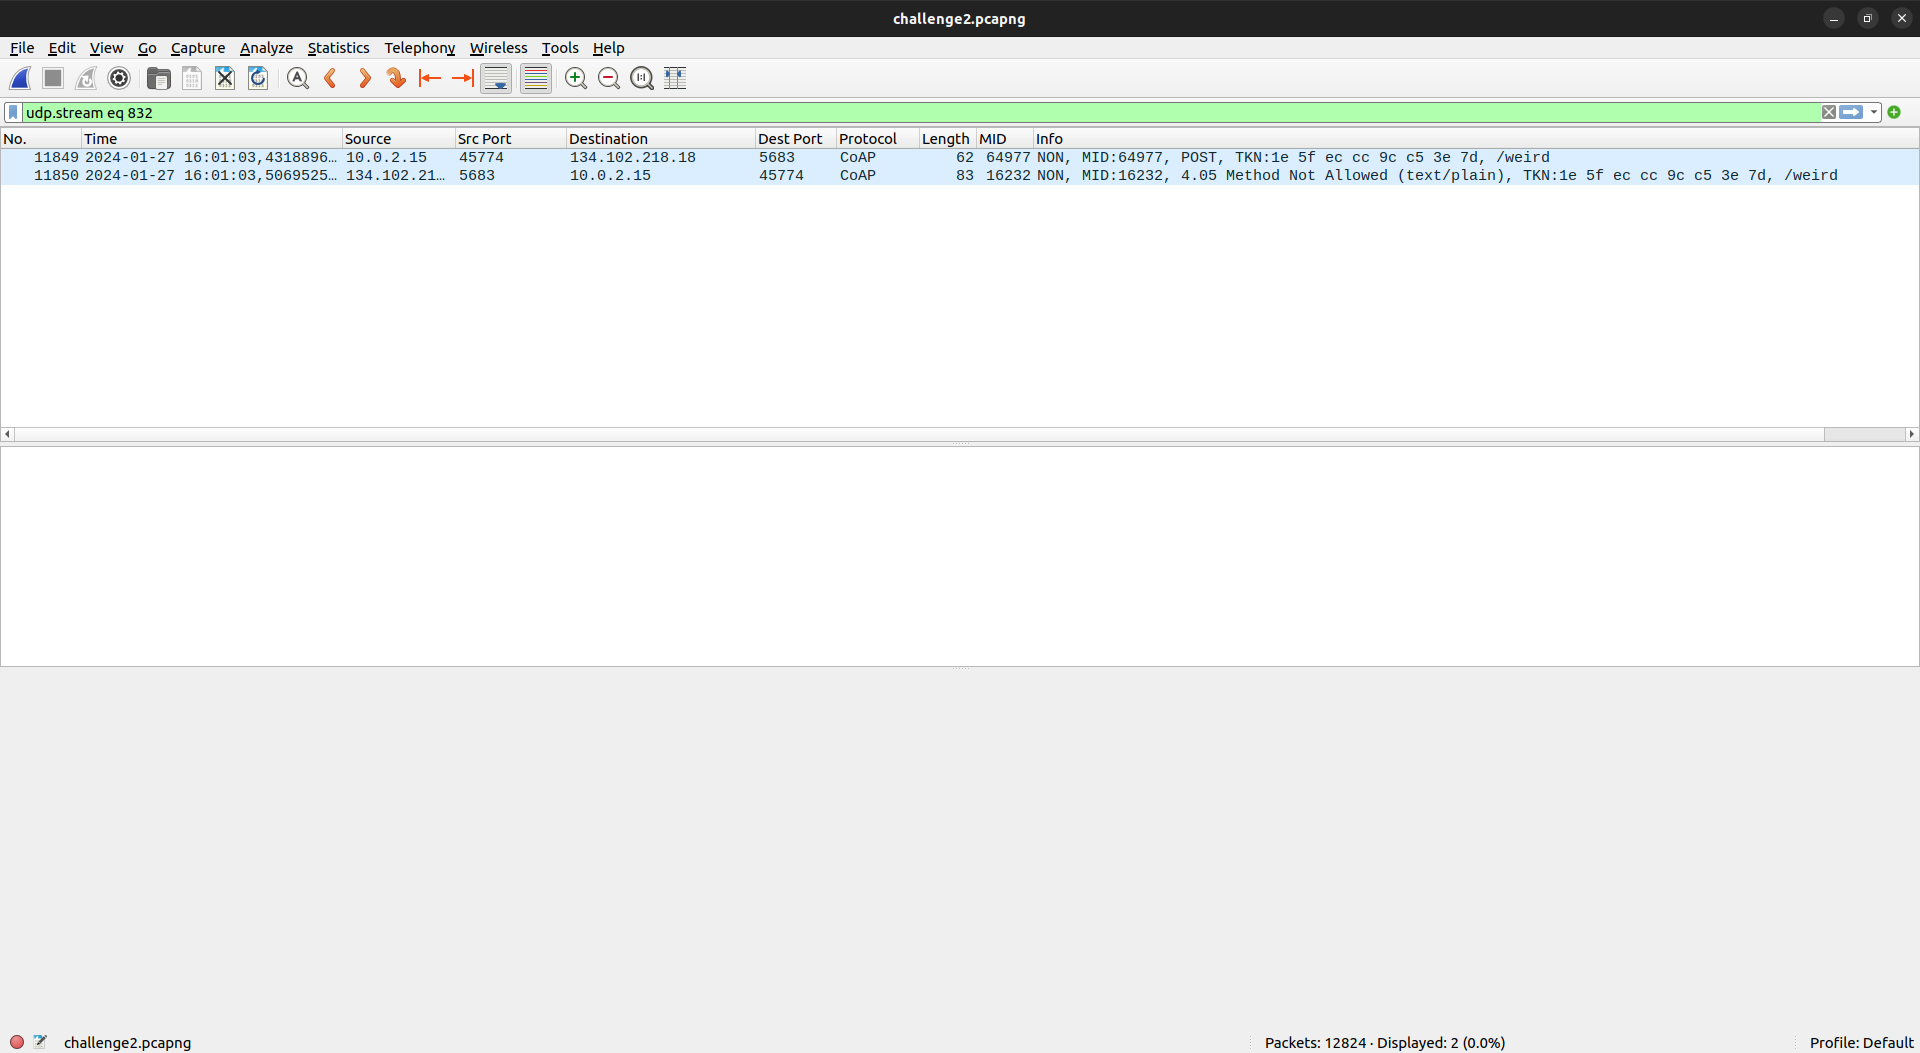
\includegraphics{2a_1.png}

    In the POST request inside a multipart request we can see that the token
is empty but the MID is the same (next image).

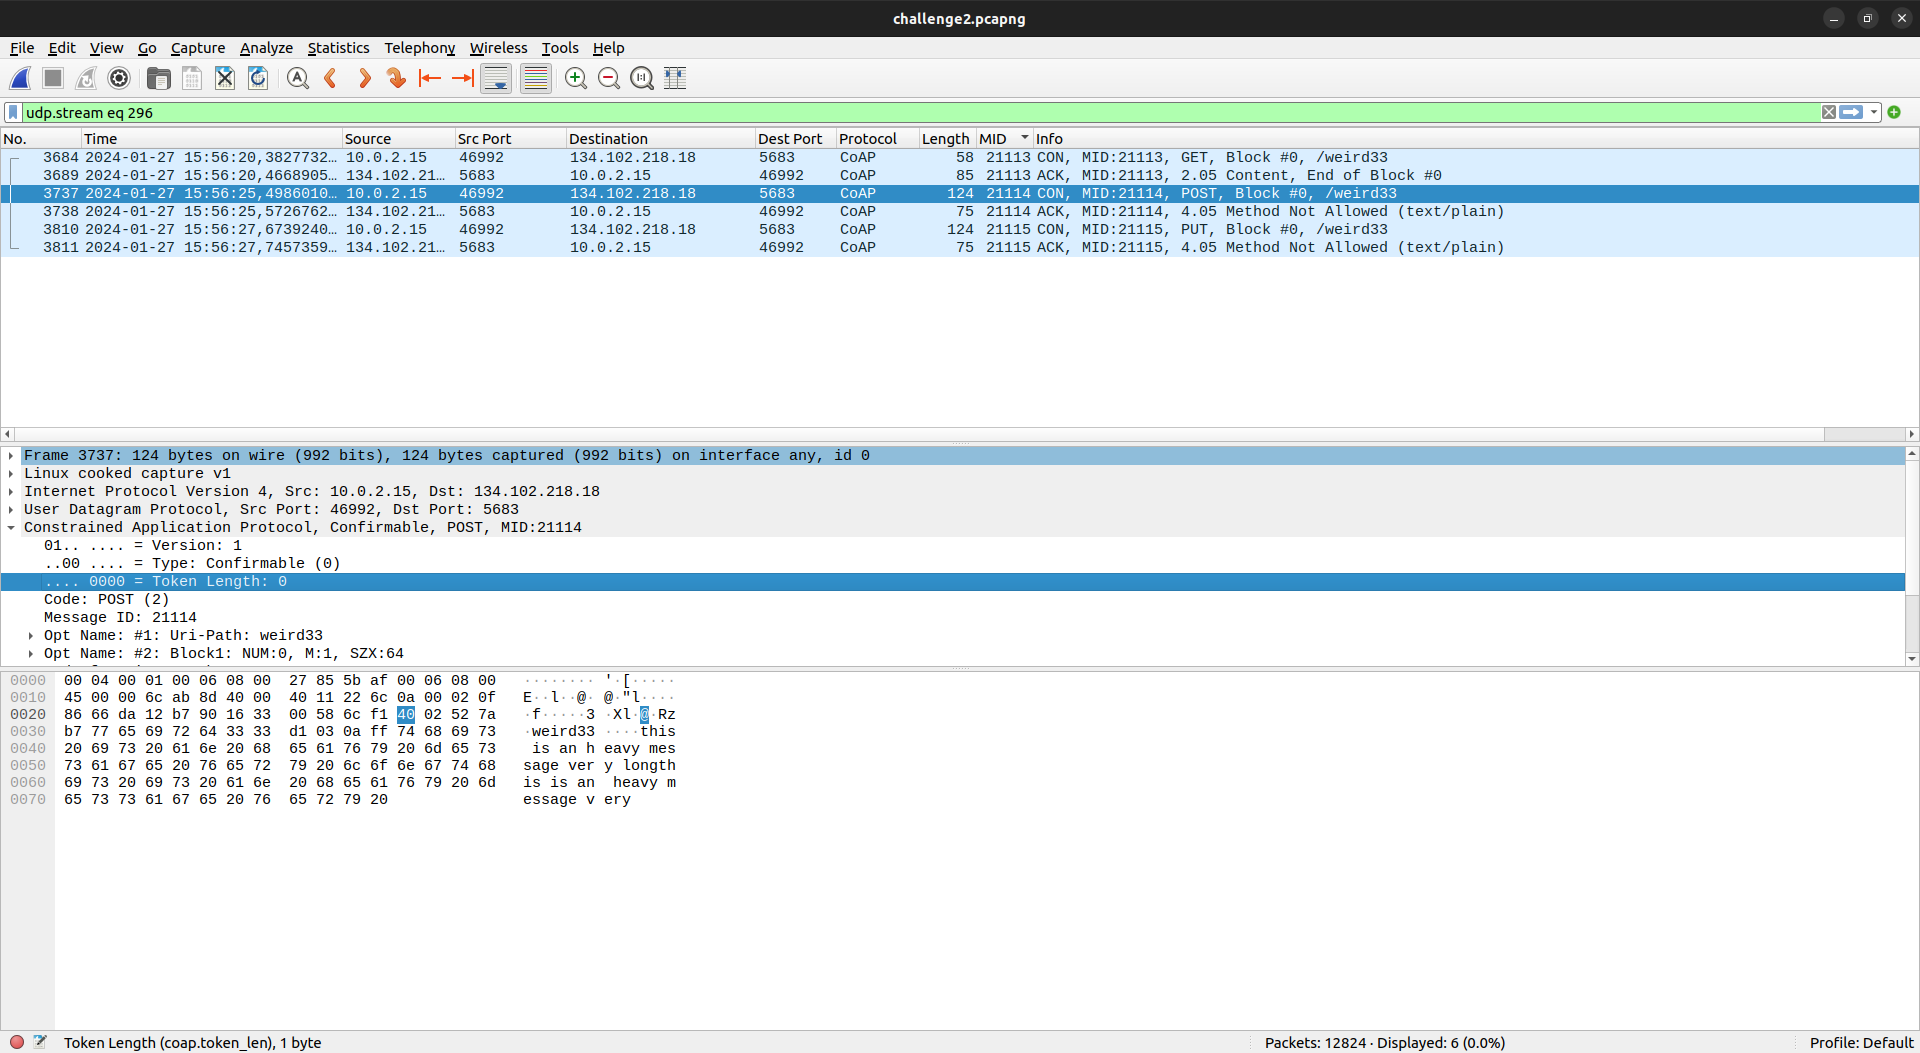
\includegraphics{2a_2.png}

    In the POST request to /hello we can see that no answer is found by
matching the token, the MID, or the UDP stream (next image).

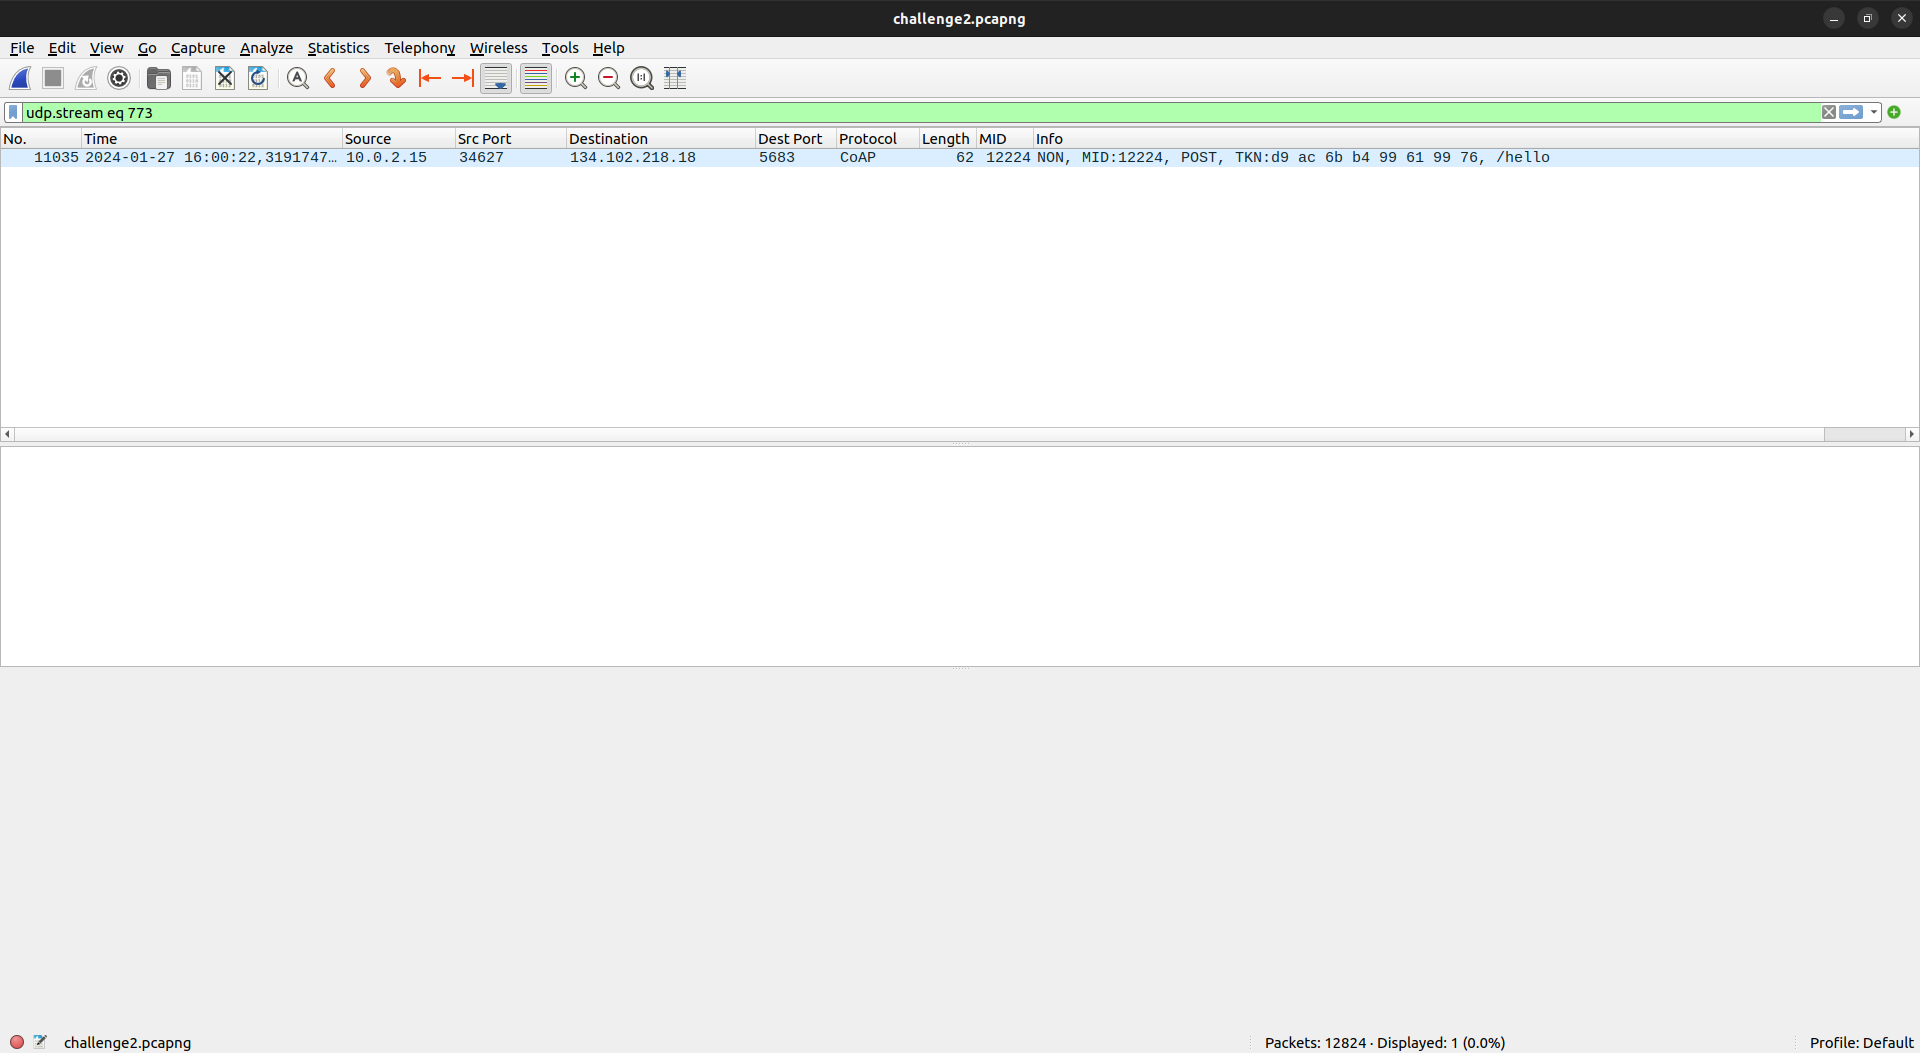
\includegraphics{2a_3.png}

    \begin{tcolorbox}[breakable, size=fbox, boxrule=1pt, pad at break*=1mm,colback=cellbackground, colframe=cellborder]
\prompt{In}{incolor}{8}{\boxspacing}
\begin{Verbatim}[commandchars=\\\{\}]
\PY{c+c1}{\PYZsh{} Find IPs of the coap.me server by looking to the DNS requests}
\PY{n}{coapme} \PY{o}{=} \PY{p}{[}\PY{p}{]}
\PY{k}{for} \PY{n}{p} \PY{o+ow}{in} \PY{n}{packets}\PY{p}{:}
    \PY{k}{if} \PY{p}{(}\PY{n}{p}\PY{o}{.}\PY{n}{haslayer}\PY{p}{(}\PY{n}{DNSRR}\PY{p}{)} \PY{c+c1}{\PYZsh{} Only DNS Resource Record packets}
        \PY{o+ow}{and} \PY{n}{p}\PY{p}{[}\PY{n}{DNSRR}\PY{p}{]}\PY{o}{.}\PY{n}{type} \PY{o}{==} \PY{l+m+mi}{1} \PY{c+c1}{\PYZsh{} Only records of type A}
        \PY{c+c1}{\PYZsh{} Only records for the coap.me server}
        \PY{o+ow}{and} \PY{n}{p}\PY{p}{[}\PY{n}{DNSRR}\PY{p}{]}\PY{o}{.}\PY{n}{rrname} \PY{o}{==} \PY{l+s+sa}{b}\PY{l+s+s1}{\PYZsq{}}\PY{l+s+s1}{coap.me.}\PY{l+s+s1}{\PYZsq{}}
    \PY{p}{)}\PY{p}{:}
        \PY{c+c1}{\PYZsh{} Save the IP of the coap.me server}
        \PY{n}{coapme}\PY{o}{.}\PY{n}{append}\PY{p}{(}\PY{n}{p}\PY{p}{[}\PY{n}{DNSRR}\PY{p}{]}\PY{o}{.}\PY{n}{rdata}\PY{p}{)}

\PY{c+c1}{\PYZsh{} Only unique IPs}
\PY{n}{coapme} \PY{o}{=} \PY{n+nb}{set}\PY{p}{(}\PY{n}{coapme}\PY{p}{)}

\PY{n+nb}{print}\PY{p}{(}\PY{l+s+s2}{\PYZdq{}}\PY{l+s+s2}{coap.me IPs:}\PY{l+s+s2}{\PYZdq{}}\PY{p}{,} \PY{n}{coapme}\PY{p}{)}
\end{Verbatim}
\end{tcolorbox}

    \begin{Verbatim}[commandchars=\\\{\}]
coap.me IPs: \{'134.102.218.18'\}
    \end{Verbatim}

    \begin{tcolorbox}[breakable, size=fbox, boxrule=1pt, pad at break*=1mm,colback=cellbackground, colframe=cellborder]
\prompt{In}{incolor}{9}{\boxspacing}
\begin{Verbatim}[commandchars=\\\{\}]
\PY{c+c1}{\PYZsh{} Find all CoAP requests to coap.me server saving the tokens}
\PY{c+c1}{\PYZsh{} that will be used to find the responses}
\PY{n}{requests\PYZus{}tokens\PYZus{}2} \PY{o}{=} \PY{p}{[}\PY{p}{]}
\PY{n}{requests\PYZus{}mids\PYZus{}2} \PY{o}{=} \PY{p}{[}\PY{p}{]}
\PY{k}{for} \PY{n}{p} \PY{o+ow}{in} \PY{n}{packets}\PY{p}{:}
    \PY{k}{if} \PY{p}{(}
        \PY{n}{p}\PY{o}{.}\PY{n}{haslayer}\PY{p}{(}\PY{n}{CoAP}\PY{p}{)} \PY{c+c1}{\PYZsh{} Only CoAP Packets}
        \PY{o+ow}{and} \PY{n}{p}\PY{p}{[}\PY{n}{CoAP}\PY{p}{]}\PY{o}{.}\PY{n}{code} \PY{o}{==} \PY{l+m+mi}{2} \PY{c+c1}{\PYZsh{} Only POST requests}
        \PY{o+ow}{and} \PY{n}{p}\PY{p}{[}\PY{n}{IP}\PY{p}{]}\PY{o}{.}\PY{n}{dst} \PY{o+ow}{in} \PY{n}{coapme} \PY{c+c1}{\PYZsh{} Only requests to the coap.me server}
    \PY{p}{)}\PY{p}{:}
        \PY{c+c1}{\PYZsh{} Block requests have empty tokens}
        \PY{k}{if} \PY{n}{p}\PY{p}{[}\PY{n}{CoAP}\PY{p}{]}\PY{o}{.}\PY{n}{token} \PY{o}{!=} \PY{l+s+sa}{b}\PY{l+s+s1}{\PYZsq{}}\PY{l+s+s1}{\PYZsq{}}\PY{p}{:}
            \PY{n}{requests\PYZus{}tokens\PYZus{}2}\PY{o}{.}\PY{n}{append}\PY{p}{(}\PY{n}{p}\PY{p}{[}\PY{n}{CoAP}\PY{p}{]}\PY{o}{.}\PY{n}{token}\PY{p}{)}

        \PY{n}{requests\PYZus{}mids\PYZus{}2}\PY{o}{.}\PY{n}{append}\PY{p}{(}\PY{n}{p}\PY{p}{[}\PY{n}{CoAP}\PY{p}{]}\PY{o}{.}\PY{n}{msg\PYZus{}id}\PY{p}{)}

\PY{n+nb}{print}\PY{p}{(}\PY{l+s+s2}{\PYZdq{}}\PY{l+s+s2}{Found }\PY{l+s+si}{\PYZpc{}d}\PY{l+s+s2}{ tokens and }\PY{l+s+si}{\PYZpc{}d}\PY{l+s+s2}{ mids of CoAP requests}\PY{l+s+s2}{\PYZdq{}}
    \PY{o}{\PYZpc{}} \PY{p}{(}\PY{n+nb}{len}\PY{p}{(}\PY{n}{requests\PYZus{}tokens\PYZus{}2}\PY{p}{)}\PY{p}{,} \PY{n+nb}{len}\PY{p}{(}\PY{n}{requests\PYZus{}mids\PYZus{}2}\PY{p}{)}\PY{p}{)}\PY{p}{)}
\end{Verbatim}
\end{tcolorbox}

    \begin{Verbatim}[commandchars=\\\{\}]
Found 27 tokens and 34 mids of CoAP requests
    \end{Verbatim}

    \begin{tcolorbox}[breakable, size=fbox, boxrule=1pt, pad at break*=1mm,colback=cellbackground, colframe=cellborder]
\prompt{In}{incolor}{10}{\boxspacing}
\begin{Verbatim}[commandchars=\\\{\}]
\PY{c+c1}{\PYZsh{} Find all CoAP responses to the previous requests}
\PY{c+c1}{\PYZsh{} searching only for the ones with a bad status code}
\PY{n}{responses\PYZus{}count\PYZus{}2} \PY{o}{=} \PY{l+m+mi}{0}
\PY{n}{bad\PYZus{}responses\PYZus{}tokens\PYZus{}2} \PY{o}{=} \PY{p}{[}\PY{p}{]}
\PY{n}{bad\PYZus{}responses\PYZus{}mids\PYZus{}2} \PY{o}{=} \PY{p}{[}\PY{p}{]}
\PY{k}{for} \PY{n}{p} \PY{o+ow}{in} \PY{n}{packets}\PY{p}{:}
    \PY{k}{if} \PY{p}{(}
        \PY{n}{p}\PY{o}{.}\PY{n}{haslayer}\PY{p}{(}\PY{n}{CoAP}\PY{p}{)}  \PY{c+c1}{\PYZsh{} Only CoAP Packets}
        \PY{o+ow}{and} \PY{n}{p}\PY{o}{.}\PY{n}{haslayer}\PY{p}{(}\PY{n}{UDP}\PY{p}{)}  \PY{c+c1}{\PYZsh{} Only UDP Packets}
        \PY{o+ow}{and} \PY{n}{p}\PY{p}{[}\PY{n}{CoAP}\PY{p}{]}\PY{o}{.}\PY{n}{code} \PY{o}{\PYZgt{}} \PY{l+m+mi}{64}  \PY{c+c1}{\PYZsh{} Only responses}
        \PY{o+ow}{and} \PY{p}{(}  \PY{c+c1}{\PYZsh{} Only responses to the previous requests}
            \PY{n}{p}\PY{p}{[}\PY{n}{CoAP}\PY{p}{]}\PY{o}{.}\PY{n}{token} \PY{o+ow}{in} \PY{n}{requests\PYZus{}tokens\PYZus{}2}  \PY{c+c1}{\PYZsh{} Check token}
            \PY{o+ow}{or} \PY{n}{p}\PY{p}{[}\PY{n}{CoAP}\PY{p}{]}\PY{o}{.}\PY{n}{msg\PYZus{}id} \PY{o+ow}{in} \PY{n}{requests\PYZus{}mids\PYZus{}2}  \PY{c+c1}{\PYZsh{} Check mid}
        \PY{p}{)}
    \PY{p}{)}\PY{p}{:}
        \PY{c+c1}{\PYZsh{} Increment the total responses count}
        \PY{n}{responses\PYZus{}count\PYZus{}2} \PY{o}{+}\PY{o}{=} \PY{l+m+mi}{1}

        \PY{c+c1}{\PYZsh{} Save bad responses}
        \PY{k}{if} \PY{n}{p}\PY{p}{[}\PY{n}{CoAP}\PY{p}{]}\PY{o}{.}\PY{n}{code} \PY{o}{\PYZgt{}} \PY{l+m+mi}{127}\PY{p}{:}
            \PY{n}{bad\PYZus{}responses\PYZus{}tokens\PYZus{}2}\PY{o}{.}\PY{n}{append}\PY{p}{(}\PY{n}{p}\PY{p}{[}\PY{n}{CoAP}\PY{p}{]}\PY{o}{.}\PY{n}{token}\PY{p}{)}
            \PY{n}{bad\PYZus{}responses\PYZus{}mids\PYZus{}2}\PY{o}{.}\PY{n}{append}\PY{p}{(}\PY{n}{p}\PY{p}{[}\PY{n}{CoAP}\PY{p}{]}\PY{o}{.}\PY{n}{msg\PYZus{}id}\PY{p}{)}

\PY{n+nb}{print}\PY{p}{(}\PY{l+s+s2}{\PYZdq{}}\PY{l+s+s2}{Found }\PY{l+s+si}{\PYZpc{}d}\PY{l+s+s2}{ responses of which }\PY{l+s+si}{\PYZpc{}d}\PY{l+s+s2}{ are bad}\PY{l+s+s2}{\PYZdq{}}
    \PY{o}{\PYZpc{}} \PY{p}{(}\PY{n}{responses\PYZus{}count\PYZus{}2}\PY{p}{,} \PY{n+nb}{len}\PY{p}{(}\PY{n}{bad\PYZus{}responses\PYZus{}mids\PYZus{}2}\PY{p}{)}\PY{p}{)}\PY{p}{)}
\end{Verbatim}
\end{tcolorbox}

    \begin{Verbatim}[commandchars=\\\{\}]
Found 33 responses of which 17 are bad
    \end{Verbatim}

    \hypertarget{question-2b}{%
\subsection{Question 2b}\label{question-2b}}

How many requests from 2a are directed to a ``weird'' resource?
(resources like /weirdXX)?

Answer: 8

The answer is given by filtering the packets, looking only for CoAP
requests related to the previous clients.

I then checked the uri\_path of each CoAP request and stored the number
of requests with the string ``weird'' in the uri\_path.

    \begin{tcolorbox}[breakable, size=fbox, boxrule=1pt, pad at break*=1mm,colback=cellbackground, colframe=cellborder]
\prompt{In}{incolor}{11}{\boxspacing}
\begin{Verbatim}[commandchars=\\\{\}]
\PY{n}{count} \PY{o}{=} \PY{l+m+mi}{0}
\PY{k}{for} \PY{n}{p} \PY{o+ow}{in} \PY{n}{packets}\PY{p}{:}
    \PY{k}{if} \PY{p}{(}
        \PY{n}{p}\PY{o}{.}\PY{n}{haslayer}\PY{p}{(}\PY{n}{CoAP}\PY{p}{)} \PY{c+c1}{\PYZsh{} Only CoAP Packets}
        \PY{o+ow}{and} \PY{p}{(}  \PY{c+c1}{\PYZsh{} Only previous requests}
            \PY{n}{p}\PY{p}{[}\PY{n}{CoAP}\PY{p}{]}\PY{o}{.}\PY{n}{token} \PY{o+ow}{in} \PY{n}{requests\PYZus{}tokens\PYZus{}2}  \PY{c+c1}{\PYZsh{} Check token}
            \PY{o+ow}{or} \PY{n}{p}\PY{p}{[}\PY{n}{CoAP}\PY{p}{]}\PY{o}{.}\PY{n}{msg\PYZus{}id} \PY{o+ow}{in} \PY{n}{requests\PYZus{}mids\PYZus{}2}  \PY{c+c1}{\PYZsh{} Check mid}
        \PY{p}{)}
    \PY{p}{)}\PY{p}{:}
        \PY{c+c1}{\PYZsh{} Check if the request has a \PYZsq{}weird\PYZsq{} segment in the Uri\PYZhy{}Path}
        \PY{n}{found} \PY{o}{=} \PY{k+kc}{False}
        \PY{k}{for} \PY{n}{option} \PY{o+ow}{in} \PY{n}{p}\PY{p}{[}\PY{n}{CoAP}\PY{p}{]}\PY{o}{.}\PY{n}{options}\PY{p}{:}
            \PY{k}{if} \PY{n}{option}\PY{p}{[}\PY{l+m+mi}{0}\PY{p}{]} \PY{o}{!=} \PY{l+s+s1}{\PYZsq{}}\PY{l+s+s1}{Uri\PYZhy{}Path}\PY{l+s+s1}{\PYZsq{}}\PY{p}{:}
                \PY{k}{continue}
            
            \PY{k}{if} \PY{l+s+sa}{b}\PY{l+s+s1}{\PYZsq{}}\PY{l+s+s1}{weird}\PY{l+s+s1}{\PYZsq{}} \PY{o+ow}{in} \PY{n}{option}\PY{p}{[}\PY{l+m+mi}{1}\PY{p}{]}\PY{p}{:}
                \PY{n}{found} \PY{o}{=} \PY{k+kc}{True}
                \PY{k}{break}
                
        \PY{c+c1}{\PYZsh{} If no \PYZsq{}weird\PYZsq{} segment is found, continue}
        \PY{k}{if} \PY{o+ow}{not} \PY{n}{found}\PY{p}{:}
            \PY{k}{continue}

        \PY{n}{count} \PY{o}{+}\PY{o}{=} \PY{l+m+mi}{1}

\PY{n}{count}
\end{Verbatim}
\end{tcolorbox}

            \begin{tcolorbox}[breakable, size=fbox, boxrule=.5pt, pad at break*=1mm, opacityfill=0]
\prompt{Out}{outcolor}{11}{\boxspacing}
\begin{Verbatim}[commandchars=\\\{\}]
8
\end{Verbatim}
\end{tcolorbox}
        
    \hypertarget{question-3a}{%
\subsection{Question 3a}\label{question-3a}}

How many MQTT Publish messages with qos=2 are RECEIVED by the clients
running in the machine capturing the traffic?

Answer: 2

The answer is given by filtering the packets, looking only for MQTT
Publish (type 3) messages with QoS set to 2.

The destination port must be different then the default one (1883) to
find received messages.

    \begin{tcolorbox}[breakable, size=fbox, boxrule=1pt, pad at break*=1mm,colback=cellbackground, colframe=cellborder]
\prompt{In}{incolor}{12}{\boxspacing}
\begin{Verbatim}[commandchars=\\\{\}]
\PY{c+c1}{\PYZsh{} Save clients and topics for next questions}
\PY{n}{clients\PYZus{}3} \PY{o}{=} \PY{p}{[}\PY{p}{]}
\PY{n}{topics\PYZus{}3} \PY{o}{=} \PY{p}{[}\PY{p}{]}

\PY{n}{count} \PY{o}{=} \PY{l+m+mi}{0}
\PY{k}{for} \PY{n}{p} \PY{o+ow}{in} \PY{n}{packets}\PY{p}{:}
    \PY{k}{if} \PY{p}{(}
        \PY{n}{p}\PY{o}{.}\PY{n}{haslayer}\PY{p}{(}\PY{n}{MQTT}\PY{p}{)} \PY{c+c1}{\PYZsh{} Only MQTT packets}
        \PY{o+ow}{and} \PY{n}{p}\PY{p}{[}\PY{n}{MQTT}\PY{p}{]}\PY{o}{.}\PY{n}{type} \PY{o}{==} \PY{l+m+mi}{3} \PY{c+c1}{\PYZsh{} Only PUBLISH packets}
        \PY{o+ow}{and} \PY{n}{p}\PY{p}{[}\PY{n}{MQTT}\PY{p}{]}\PY{o}{.}\PY{n}{QOS} \PY{o}{==} \PY{l+m+mi}{2} \PY{c+c1}{\PYZsh{} Only QoS 2 packets}
        \PY{o+ow}{and} \PY{n}{p}\PY{p}{[}\PY{n}{TCP}\PY{p}{]}\PY{o}{.}\PY{n}{dport} \PY{o}{!=} \PY{l+m+mi}{1883} \PY{c+c1}{\PYZsh{} Only packets received by clients}
    \PY{p}{)}\PY{p}{:}
        \PY{n}{count} \PY{o}{+}\PY{o}{=} \PY{l+m+mi}{1}
        \PY{n}{clients\PYZus{}3}\PY{o}{.}\PY{n}{append}\PY{p}{(}\PY{n}{p}\PY{p}{[}\PY{n}{TCP}\PY{p}{]}\PY{o}{.}\PY{n}{dport}\PY{p}{)}
        \PY{n}{topics\PYZus{}3}\PY{o}{.}\PY{n}{append}\PY{p}{(}\PY{n}{p}\PY{p}{[}\PY{n}{MQTT}\PY{p}{]}\PY{o}{.}\PY{n}{topic}\PY{p}{)}

\PY{n}{count}
\end{Verbatim}
\end{tcolorbox}

            \begin{tcolorbox}[breakable, size=fbox, boxrule=.5pt, pad at break*=1mm, opacityfill=0]
\prompt{Out}{outcolor}{12}{\boxspacing}
\begin{Verbatim}[commandchars=\\\{\}]
2
\end{Verbatim}
\end{tcolorbox}
        
    \hypertarget{question-3b}{%
\subsection{Question 3b}\label{question-3b}}

How many clients are involved in the messages found in 3a?

Answer: 1

The answer is given by counting the number of unique clients (ports)
that were found in the previous question.

    \begin{tcolorbox}[breakable, size=fbox, boxrule=1pt, pad at break*=1mm,colback=cellbackground, colframe=cellborder]
\prompt{In}{incolor}{13}{\boxspacing}
\begin{Verbatim}[commandchars=\\\{\}]
\PY{n}{clients\PYZus{}3} \PY{o}{=} \PY{n+nb}{set}\PY{p}{(}\PY{n}{clients\PYZus{}3}\PY{p}{)}
\PY{n+nb}{len}\PY{p}{(}\PY{n}{clients\PYZus{}3}\PY{p}{)}
\end{Verbatim}
\end{tcolorbox}

            \begin{tcolorbox}[breakable, size=fbox, boxrule=.5pt, pad at break*=1mm, opacityfill=0]
\prompt{Out}{outcolor}{13}{\boxspacing}
\begin{Verbatim}[commandchars=\\\{\}]
1
\end{Verbatim}
\end{tcolorbox}
        
    \hypertarget{question-3c}{%
\subsection{Question 3c}\label{question-3c}}

What are the MQTT Message identifiers (ID) of the subscribe requests
that let the client receive the messages found in 3a?

Answer: 15

The answer is given by filtering the packets, looking only for MQTT
Subscribe (type 8) messages that are related to the previous clients.

Each subscribe message then must be checked to see if it is related to
the previous topics.

In particular the topics of the previous publish messages are:

\begin{itemize}
\tightlist
\item
  hospital/facility2/section0
\item
  hospital/facility2/room4/temperature
\end{itemize}

Because there is only one client and there are many combinations to
check I used Wireshark to find the answer.

\begin{verbatim}
mqtt and mqtt.msgtype == 8 and tcp.srcport == 59385 and tcp.dstport == 1883
\end{verbatim}

Possible valid combinations:

\begin{itemize}
\tightlist
\item
  hospital/\#
\item
  hospital/facility2/\#
\item
  hospital/facility2/room4/+
\item
  hospital/+/room4/temperature
\item
  hospital/facility2/section0
\item
  hospital/+/section0
\item
  \ldots{}
\end{itemize}

In the end, only the subscribe message with the topic hospital/\# and ID
15 was found.

    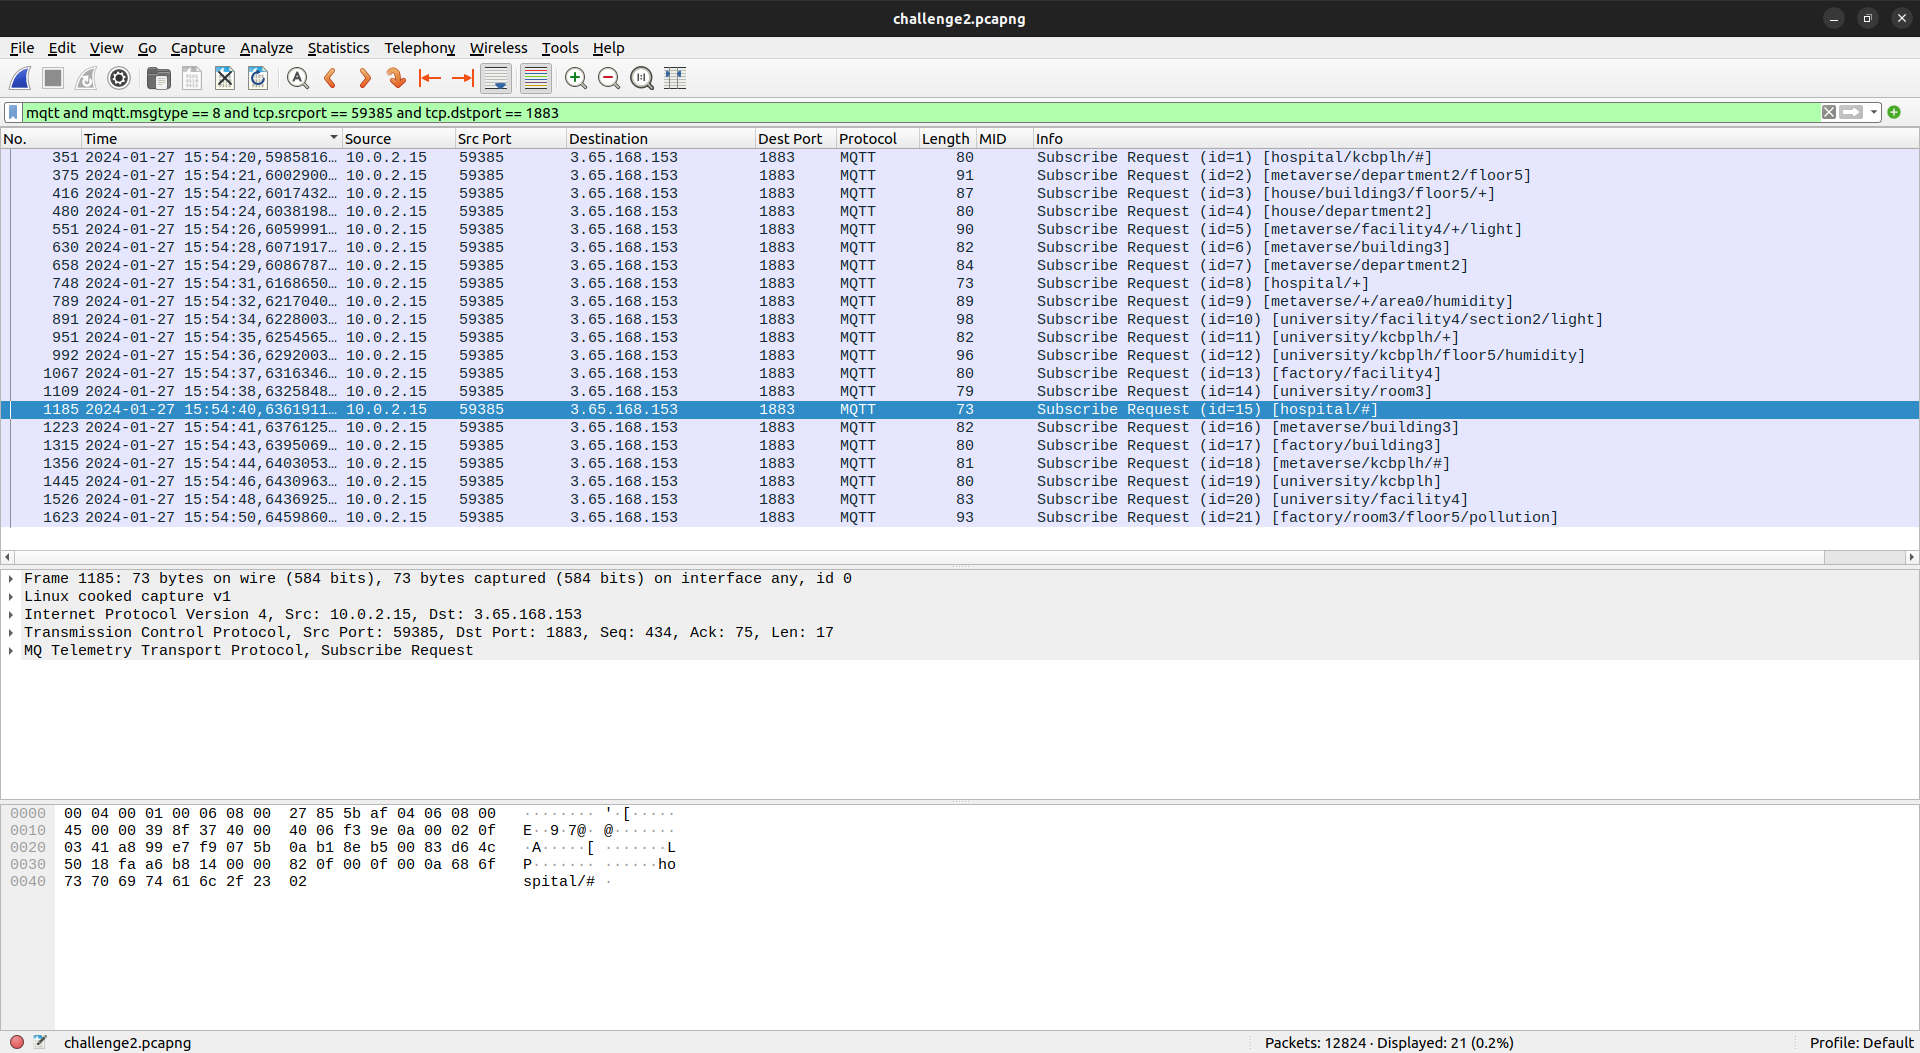
\includegraphics{3c.png}

    \begin{tcolorbox}[breakable, size=fbox, boxrule=1pt, pad at break*=1mm,colback=cellbackground, colframe=cellborder]
\prompt{In}{incolor}{14}{\boxspacing}
\begin{Verbatim}[commandchars=\\\{\}]
\PY{n}{topics\PYZus{}3}
\end{Verbatim}
\end{tcolorbox}

            \begin{tcolorbox}[breakable, size=fbox, boxrule=.5pt, pad at break*=1mm, opacityfill=0]
\prompt{Out}{outcolor}{14}{\boxspacing}
\begin{Verbatim}[commandchars=\\\{\}]
[b'hospital/facility2/section0', b'hospital/facility2/room4/temperature']
\end{Verbatim}
\end{tcolorbox}
        
    \begin{tcolorbox}[breakable, size=fbox, boxrule=1pt, pad at break*=1mm,colback=cellbackground, colframe=cellborder]
\prompt{In}{incolor}{15}{\boxspacing}
\begin{Verbatim}[commandchars=\\\{\}]
\PY{n}{clients\PYZus{}3}
\end{Verbatim}
\end{tcolorbox}

            \begin{tcolorbox}[breakable, size=fbox, boxrule=.5pt, pad at break*=1mm, opacityfill=0]
\prompt{Out}{outcolor}{15}{\boxspacing}
\begin{Verbatim}[commandchars=\\\{\}]
\{59385\}
\end{Verbatim}
\end{tcolorbox}
        
    \hypertarget{question-4a}{%
\subsection{Question 4a}\label{question-4a}}

How many MQTT clients sent a subscribe message to a public broker using
at least one wildcard?

Answer: 4

The answer is given by filtering the packets, looking only for MQTT
Subscribe (type 8) messages that are related to a public broker.

This is done by checking the destination IP of the packets to be
different from the local IP.

Then each subscribe message must be checked to see if it contains a
wildcard `+' or `\#'.

    \begin{tcolorbox}[breakable, size=fbox, boxrule=1pt, pad at break*=1mm,colback=cellbackground, colframe=cellborder]
\prompt{In}{incolor}{31}{\boxspacing}
\begin{Verbatim}[commandchars=\\\{\}]
\PY{c+c1}{\PYZsh{} Save topics for next questions}
\PY{n}{topics\PYZus{}4} \PY{o}{=} \PY{p}{[}\PY{p}{]}
\PY{n}{clients\PYZus{}4} \PY{o}{=} \PY{p}{[}\PY{p}{]}
\PY{k}{for} \PY{n}{p} \PY{o+ow}{in} \PY{n}{packets}\PY{p}{:}
    \PY{k}{if} \PY{p}{(}
        \PY{n}{p}\PY{o}{.}\PY{n}{haslayer}\PY{p}{(}\PY{n}{MQTT}\PY{p}{)} \PY{c+c1}{\PYZsh{} Only MQTT packets}
        \PY{o+ow}{and} \PY{n}{p}\PY{p}{[}\PY{n}{MQTT}\PY{p}{]}\PY{o}{.}\PY{n}{type} \PY{o}{==} \PY{l+m+mi}{8} \PY{c+c1}{\PYZsh{} Only SUBSCRIBE packets}
        \PY{o+ow}{and} \PY{n}{p}\PY{p}{[}\PY{n}{TCP}\PY{p}{]}\PY{o}{.}\PY{n}{dport} \PY{o}{==} \PY{l+m+mi}{1883} \PY{c+c1}{\PYZsh{} Only packets to the MQTT Broker}
        \PY{o+ow}{and} \PY{n}{p}\PY{p}{[}\PY{n}{IP}\PY{p}{]}\PY{o}{.}\PY{n}{dst} \PY{o}{!=} \PY{l+s+s2}{\PYZdq{}}\PY{l+s+s2}{127.0.0.1}\PY{l+s+s2}{\PYZdq{}} \PY{c+c1}{\PYZsh{} Only packets not to localhost}
        \PY{o+ow}{and} \PY{n}{p}\PY{o}{.}\PY{n}{haslayer}\PY{p}{(}\PY{n}{MQTTTopicQOS}\PY{p}{)} \PY{c+c1}{\PYZsh{} Only packets with a list of topics}
    \PY{p}{)}\PY{p}{:}
        \PY{c+c1}{\PYZsh{} Check if the topic has at least one wildcard}
        \PY{n}{found} \PY{o}{=} \PY{k+kc}{False}
        \PY{k}{for} \PY{n}{topic} \PY{o+ow}{in} \PY{n}{p}\PY{p}{[}\PY{n}{MQTTSubscribe}\PY{p}{]}\PY{o}{.}\PY{n}{topics}\PY{p}{:}
            \PY{n}{t} \PY{o}{=} \PY{n}{topic}\PY{p}{[}\PY{n}{MQTTTopicQOS}\PY{p}{]}\PY{o}{.}\PY{n}{topic}
            \PY{k}{if} \PY{l+s+sa}{b}\PY{l+s+s1}{\PYZsq{}}\PY{l+s+s1}{+}\PY{l+s+s1}{\PYZsq{}} \PY{o+ow}{in} \PY{n}{t} \PY{o+ow}{or} \PY{l+s+sa}{b}\PY{l+s+s1}{\PYZsq{}}\PY{l+s+s1}{\PYZsh{}}\PY{l+s+s1}{\PYZsq{}} \PY{o+ow}{in} \PY{n}{t}\PY{p}{:}
                \PY{c+c1}{\PYZsh{} In some topics the length of the topics}
                \PY{c+c1}{\PYZsh{} and the topic itself are different}
                \PY{c+c1}{\PYZsh{} Probably there is something wrong with the parsing}
                \PY{c+c1}{\PYZsh{} This is an issue for the next questions}
                \PY{c+c1}{\PYZsh{} l = topic[MQTTTopicQOS].length}
                \PY{c+c1}{\PYZsh{} print(t, l, len(t) == l)}
                \PY{n}{topics\PYZus{}4}\PY{o}{.}\PY{n}{append}\PY{p}{(}\PY{n}{t}\PY{p}{)}
                \PY{n}{found} \PY{o}{=} \PY{k+kc}{True}
                \PY{k}{break}
                
        \PY{k}{if} \PY{o+ow}{not} \PY{n}{found}\PY{p}{:}
            \PY{k}{continue}
        
        \PY{n}{clients\PYZus{}4}\PY{o}{.}\PY{n}{append}\PY{p}{(}\PY{n}{p}\PY{p}{[}\PY{n}{TCP}\PY{p}{]}\PY{o}{.}\PY{n}{sport}\PY{p}{)}

\PY{c+c1}{\PYZsh{} Only unique clients}
\PY{n}{clients\PYZus{}4} \PY{o}{=} \PY{n+nb}{set}\PY{p}{(}\PY{n}{clients\PYZus{}4}\PY{p}{)}

\PY{n+nb}{len}\PY{p}{(}\PY{n}{clients\PYZus{}4}\PY{p}{)}
\end{Verbatim}
\end{tcolorbox}

            \begin{tcolorbox}[breakable, size=fbox, boxrule=.5pt, pad at break*=1mm, opacityfill=0]
\prompt{Out}{outcolor}{31}{\boxspacing}
\begin{Verbatim}[commandchars=\\\{\}]
4
\end{Verbatim}
\end{tcolorbox}
        
    If we use Wireshark we could find the same result by applying the
following filter:

\begin{verbatim}
mqtt and mqtt.msgtype == 8 and tcp.dstport == 1883 and ip.dst != 127.0.0.1 
    and (mqtt.topic contains "+" or mqtt.topic contains "#")
\end{verbatim}

\begin{figure}
\centering
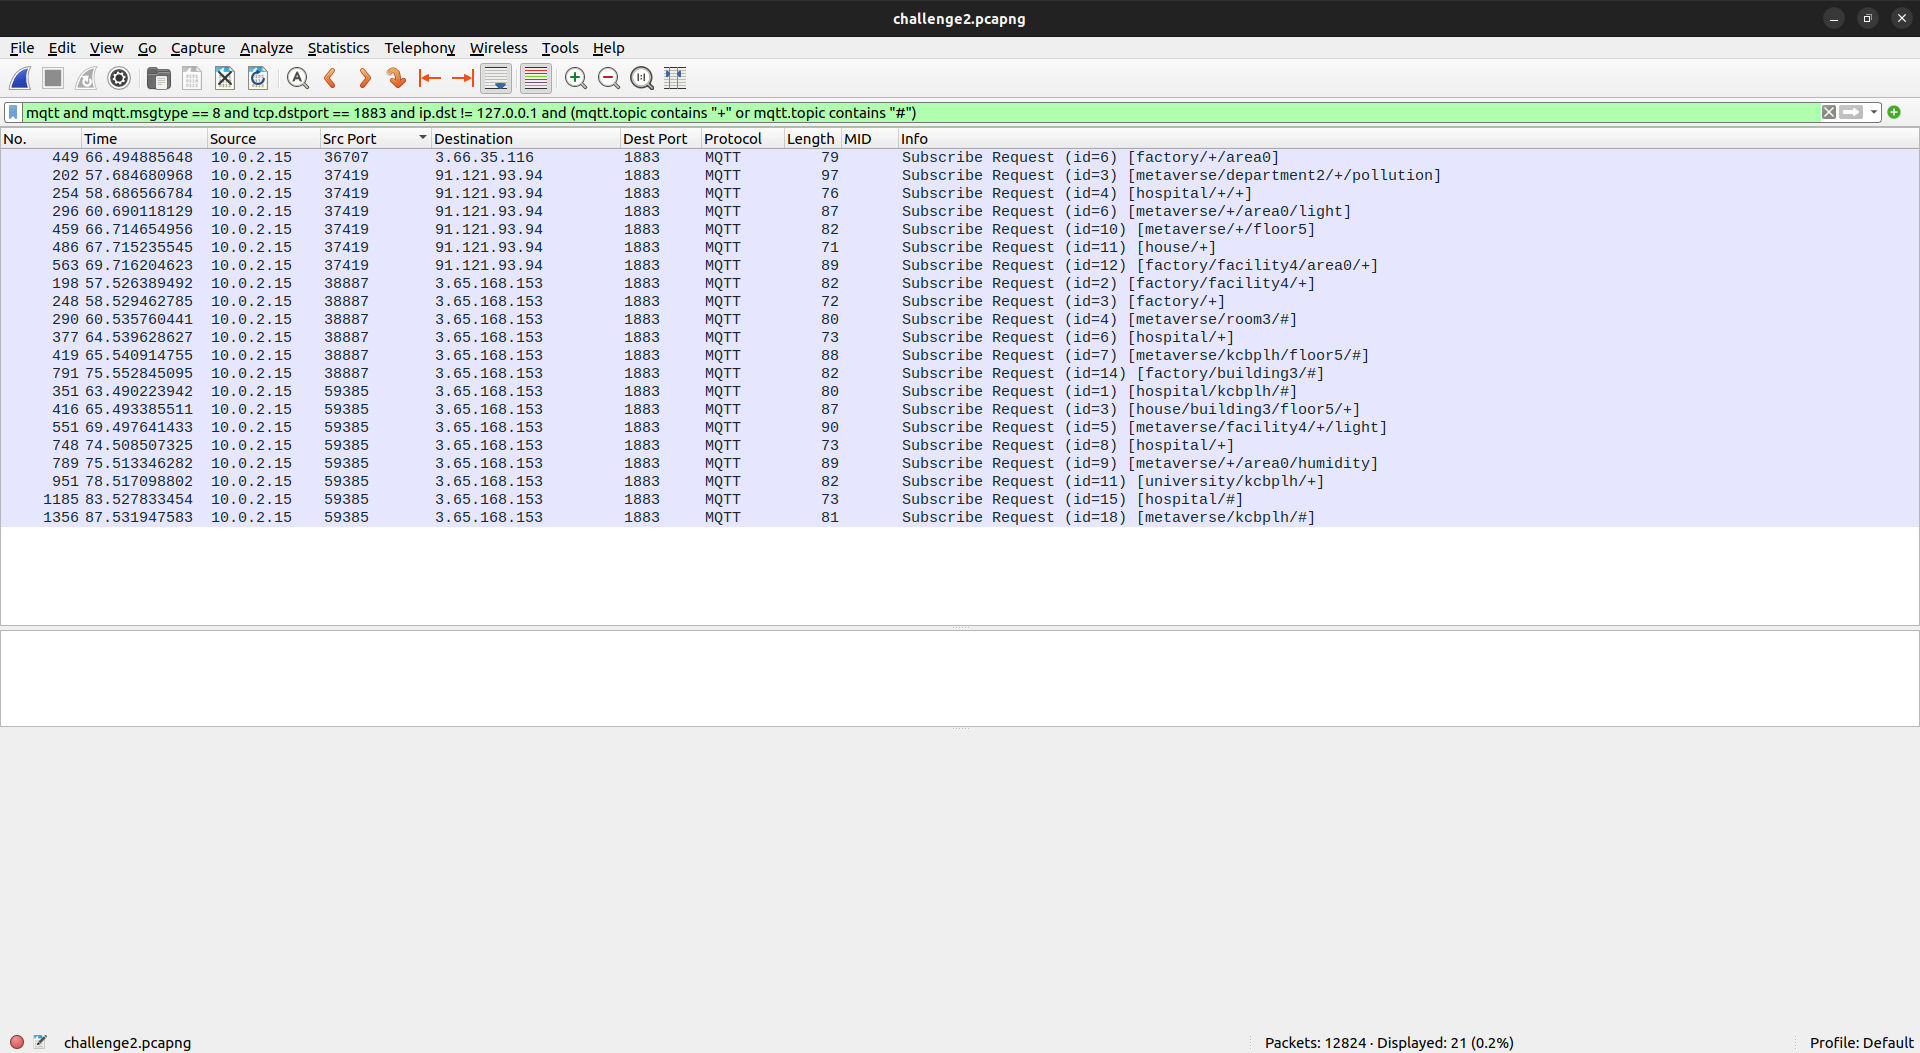
\includegraphics{4a.png}
\caption{picture}
\end{figure}

    \hypertarget{question-4b}{%
\subsection{Question 4b}\label{question-4b}}

Considering clients found in 4a, how many of them WOULD receive a
publish message directed to the topic:
``metaverse/facility4/area0/light''?

Answer: 2

Only the subscribe requests with topic
\texttt{metaverse/facility4/+/light} and
\texttt{metaverse/+/area0/light} from two different clients will receive
a publish message about \texttt{metaverse/facility4/area0/light}

There is a problem in Scapy for parsing the topics, so the answer was
found by using Wireshark.

    \begin{tcolorbox}[breakable, size=fbox, boxrule=1pt, pad at break*=1mm,colback=cellbackground, colframe=cellborder]
\prompt{In}{incolor}{17}{\boxspacing}
\begin{Verbatim}[commandchars=\\\{\}]
\PY{c+c1}{\PYZsh{} List of topics from previous question}
\PY{c+c1}{\PYZsh{} Some of them are malformed with not printable characters}
\PY{k}{for} \PY{n}{t} \PY{o+ow}{in} \PY{n}{topics\PYZus{}4}\PY{p}{:}
    \PY{n+nb}{print}\PY{p}{(}\PY{n}{t}\PY{p}{)}
\end{Verbatim}
\end{tcolorbox}

    \begin{Verbatim}[commandchars=\\\{\}]
b'factory/facility4/+'
b'taverse/department2/+/pollution\textbackslash{}x01'
b'factory/+'
b'spital/+/+\textbackslash{}x00'
b'metaverse/room3/\#'
b'taverse/+/area0/light\textbackslash{}x01'
b'hospital/kcbplh/\#'
b'hospital/+'
b'house/building3/floor5/+'
b'metaverse/kcbplh/floor5/\#'
b'ctory/+/area0\textbackslash{}x00'
b'taverse/+/floor5\textbackslash{}x01'
b'use/+\textbackslash{}x02'
b'metaverse/facility4/+/light'
b'ctory/facility4/area0/+\textbackslash{}x02'
b'hospital/+'
b'metaverse/+/area0/humidity'
b'factory/building3/\#'
b'university/kcbplh/+'
b'hospital/\#'
b'metaverse/kcbplh/\#'
    \end{Verbatim}

    Using the same filter of the previous question, we can see that there
are only two possible topics that satisfy the request:

\begin{itemize}
\tightlist
\item
  metaverse/facility4/+/light
\item
  metaverse/+/area0/light
\end{itemize}

\begin{figure}
\centering
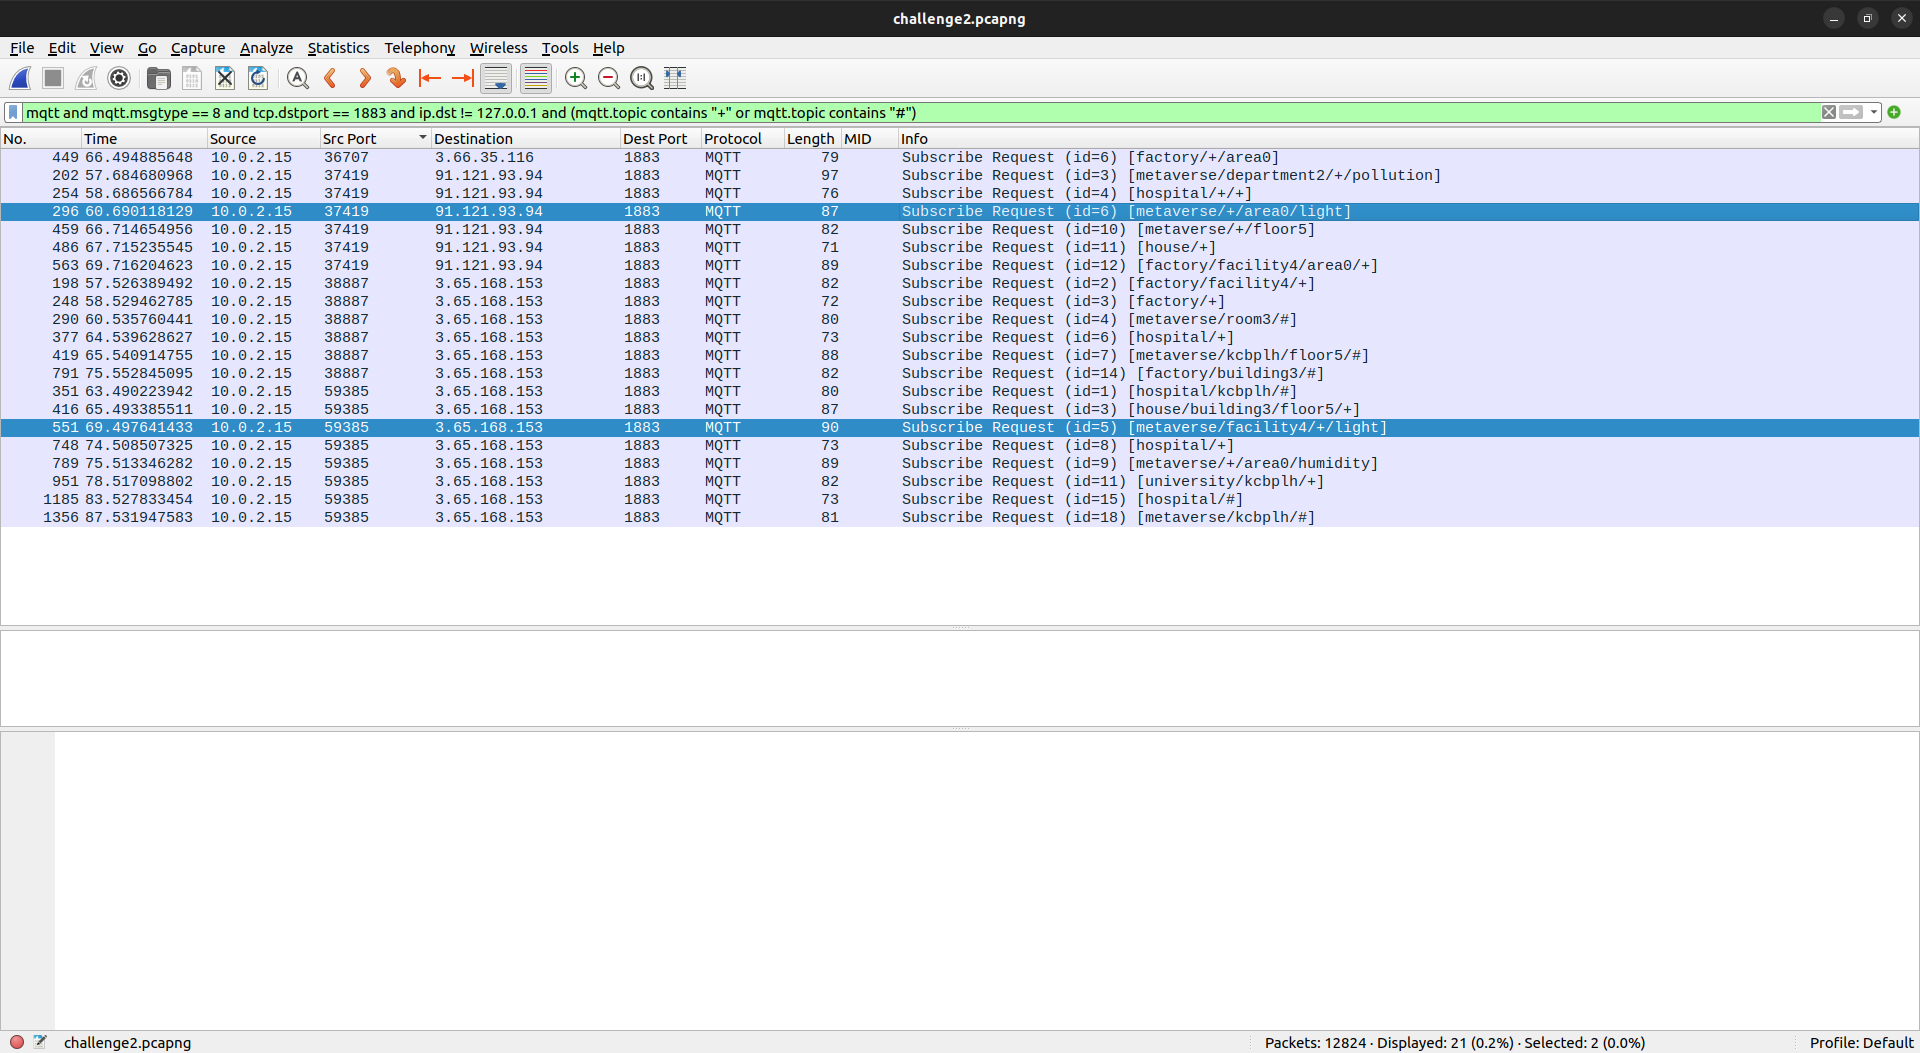
\includegraphics{4b.png}
\caption{picture}
\end{figure}

    \hypertarget{question-5}{%
\subsection{Question 5}\label{question-5}}

How many MQTT ACK messages in total are received by clients who
connected to brokers specifying a client identifier shorter than 15
bytes and using MQTT version 3.1.1?

Answer: 233

The answer is given by first finding all the clients that have sent a
CONNECT message with a client id shorter than 15 bytes and MQTT version
3.1.1

After that we have to directly count all the ACK messages that are
received by these clients.

I didn't consider if the clients have done multiple connections with
different ids.

Instead, I interpreted it as if at least one connection was done as
required than count all the ACK messages for these clients.

For the ACK messages I considered the following types:

\begin{longtable}[]{@{}ll@{}}
\toprule
msg & type\tabularnewline
\midrule
\endhead
CONNACK & 2\tabularnewline
PUBACK & 4\tabularnewline
PUBREC & 5\tabularnewline
PUBREL & 6\tabularnewline
PUBCOMP & 7\tabularnewline
SUBACK & 9\tabularnewline
UNSUBACK & 11\tabularnewline
\bottomrule
\end{longtable}

    \begin{tcolorbox}[breakable, size=fbox, boxrule=1pt, pad at break*=1mm,colback=cellbackground, colframe=cellborder]
\prompt{In}{incolor}{18}{\boxspacing}
\begin{Verbatim}[commandchars=\\\{\}]
\PY{c+c1}{\PYZsh{} Save clients between first and second filter}
\PY{n}{clients\PYZus{}5} \PY{o}{=} \PY{p}{[}\PY{p}{]}

\PY{c+c1}{\PYZsh{} We need to find first all the clients that have connected to a MQTT broker}
\PY{c+c1}{\PYZsh{} with a client id that is shorter than 15 bytes and using MQTT version 3.1.1.}
\PY{k}{for} \PY{n}{p} \PY{o+ow}{in} \PY{n}{packets}\PY{p}{:}
    \PY{k}{if} \PY{p}{(}
        \PY{n}{p}\PY{o}{.}\PY{n}{haslayer}\PY{p}{(}\PY{n}{MQTT}\PY{p}{)} \PY{c+c1}{\PYZsh{} Only MQTT packets}
        \PY{o+ow}{and} \PY{n}{p}\PY{o}{.}\PY{n}{haslayer}\PY{p}{(}\PY{n}{MQTTConnect}\PY{p}{)} \PY{c+c1}{\PYZsh{} Only connect packets}
        \PY{o+ow}{and} \PY{n}{p}\PY{p}{[}\PY{n}{MQTTConnect}\PY{p}{]}\PY{o}{.}\PY{n}{protolevel} \PY{o}{==} \PY{l+m+mi}{4} \PY{c+c1}{\PYZsh{} Check MQTT version to be 3.1.1 (4)}
        \PY{o+ow}{and} \PY{n+nb}{len}\PY{p}{(}\PY{n}{p}\PY{p}{[}\PY{n}{MQTTConnect}\PY{p}{]}\PY{o}{.}\PY{n}{clientId}\PY{p}{)} \PY{o}{\PYZlt{}} \PY{l+m+mi}{15}
    \PY{p}{)}\PY{p}{:}
        \PY{n}{clients\PYZus{}5}\PY{o}{.}\PY{n}{append}\PY{p}{(}\PY{n}{p}\PY{p}{[}\PY{n}{TCP}\PY{p}{]}\PY{o}{.}\PY{n}{sport}\PY{p}{)}

\PY{c+c1}{\PYZsh{} Only unique clients}
\PY{n}{clients\PYZus{}5} \PY{o}{=} \PY{n+nb}{set}\PY{p}{(}\PY{n}{clients\PYZus{}5}\PY{p}{)}

\PY{n+nb}{print}\PY{p}{(}\PY{l+s+s2}{\PYZdq{}}\PY{l+s+s2}{Found }\PY{l+s+si}{\PYZpc{}d}\PY{l+s+s2}{ clients}\PY{l+s+s2}{\PYZdq{}} \PY{o}{\PYZpc{}} \PY{n+nb}{len}\PY{p}{(}\PY{n}{clients\PYZus{}5}\PY{p}{)}\PY{p}{)}
\end{Verbatim}
\end{tcolorbox}

    \begin{Verbatim}[commandchars=\\\{\}]
Found 2 clients
    \end{Verbatim}

    \begin{tcolorbox}[breakable, size=fbox, boxrule=1pt, pad at break*=1mm,colback=cellbackground, colframe=cellborder]
\prompt{In}{incolor}{19}{\boxspacing}
\begin{Verbatim}[commandchars=\\\{\}]
\PY{c+c1}{\PYZsh{} Once we have the right clients, we can simply count the number}
\PY{c+c1}{\PYZsh{} of ACK packets that are sent by a MQTT Broker to these clients}
\PY{n}{count} \PY{o}{=} \PY{l+m+mi}{0}
\PY{k}{for} \PY{n}{p} \PY{o+ow}{in} \PY{n}{packets}\PY{p}{:}
    \PY{k}{if} \PY{p}{(}
        \PY{n}{p}\PY{o}{.}\PY{n}{haslayer}\PY{p}{(}\PY{n}{MQTT}\PY{p}{)} \PY{c+c1}{\PYZsh{} Only MQTT packets}
        \PY{o+ow}{and} \PY{n}{p}\PY{p}{[}\PY{n}{MQTT}\PY{p}{]}\PY{o}{.}\PY{n}{type} \PY{o+ow}{in} \PY{p}{[}\PY{l+m+mi}{2}\PY{p}{,} \PY{l+m+mi}{4}\PY{p}{,} \PY{l+m+mi}{5}\PY{p}{,} \PY{l+m+mi}{6}\PY{p}{,} \PY{l+m+mi}{7}\PY{p}{,} \PY{l+m+mi}{9}\PY{p}{,} \PY{l+m+mi}{11}\PY{p}{]} \PY{c+c1}{\PYZsh{} Only ACK packets}
        \PY{o+ow}{and} \PY{n}{p}\PY{p}{[}\PY{n}{TCP}\PY{p}{]}\PY{o}{.}\PY{n}{dport} \PY{o+ow}{in} \PY{n}{clients\PYZus{}5} \PY{c+c1}{\PYZsh{} Only packets to the clients}
    \PY{p}{)}\PY{p}{:} 
        \PY{n}{count} \PY{o}{+}\PY{o}{=} \PY{l+m+mi}{1}

\PY{n}{count}
\end{Verbatim}
\end{tcolorbox}

            \begin{tcolorbox}[breakable, size=fbox, boxrule=.5pt, pad at break*=1mm, opacityfill=0]
\prompt{Out}{outcolor}{19}{\boxspacing}
\begin{Verbatim}[commandchars=\\\{\}]
233
\end{Verbatim}
\end{tcolorbox}
        
    \hypertarget{question-6a}{%
\subsection{Question 6a}\label{question-6a}}

How many MQTT subscribe requests with message ID=1 are directed to the
HiveMQ broker?

Answer: 3

The answer is given by first finding all the IPs of the HiveMQ broker.

In order to find them, we have to check all DNS resource records for
``broker.hivemq.com'' and saving the related IPs.

After that, we have to find all the MQTT subscribe requests with message
ID=1 and directed to one of the IPs found before.

    \begin{tcolorbox}[breakable, size=fbox, boxrule=1pt, pad at break*=1mm,colback=cellbackground, colframe=cellborder]
\prompt{In}{incolor}{20}{\boxspacing}
\begin{Verbatim}[commandchars=\\\{\}]
\PY{c+c1}{\PYZsh{} Find IPs of the HiveMQ server by looking to the DNS requests}
\PY{n}{hivemq} \PY{o}{=} \PY{p}{[}\PY{p}{]}
\PY{k}{for} \PY{n}{p} \PY{o+ow}{in} \PY{n}{packets}\PY{p}{:}
    \PY{k}{if} \PY{p}{(}
        \PY{n}{p}\PY{o}{.}\PY{n}{haslayer}\PY{p}{(}\PY{n}{DNSRR}\PY{p}{)} \PY{c+c1}{\PYZsh{} Only DNS Resource Record packets}
        \PY{o+ow}{and} \PY{n}{p}\PY{p}{[}\PY{n}{DNSRR}\PY{p}{]}\PY{o}{.}\PY{n}{type} \PY{o}{==} \PY{l+m+mi}{1} \PY{c+c1}{\PYZsh{} Only records of type A}
        \PY{c+c1}{\PYZsh{} Only records for the HiveMQ server}
        \PY{o+ow}{and} \PY{n}{p}\PY{p}{[}\PY{n}{DNSRR}\PY{p}{]}\PY{o}{.}\PY{n}{rrname} \PY{o}{==} \PY{l+s+sa}{b}\PY{l+s+s1}{\PYZsq{}}\PY{l+s+s1}{broker.hivemq.com.}\PY{l+s+s1}{\PYZsq{}}
    \PY{p}{)}\PY{p}{:}
        \PY{c+c1}{\PYZsh{} Save the IP of the coap.me server}
        \PY{n}{hivemq}\PY{o}{.}\PY{n}{append}\PY{p}{(}\PY{n}{p}\PY{p}{[}\PY{n}{DNSRR}\PY{p}{]}\PY{o}{.}\PY{n}{rdata}\PY{p}{)}

\PY{c+c1}{\PYZsh{} Only unique IPs}
\PY{n}{hivemq} \PY{o}{=} \PY{n+nb}{set}\PY{p}{(}\PY{n}{hivemq}\PY{p}{)}

\PY{n+nb}{print}\PY{p}{(}\PY{l+s+s2}{\PYZdq{}}\PY{l+s+s2}{HiveMQ IPs:}\PY{l+s+s2}{\PYZdq{}}\PY{p}{,} \PY{n}{hivemq}\PY{p}{)}
\end{Verbatim}
\end{tcolorbox}

    \begin{Verbatim}[commandchars=\\\{\}]
HiveMQ IPs: \{'3.65.168.153', '3.66.35.116'\}
    \end{Verbatim}

    \begin{tcolorbox}[breakable, size=fbox, boxrule=1pt, pad at break*=1mm,colback=cellbackground, colframe=cellborder]
\prompt{In}{incolor}{21}{\boxspacing}
\begin{Verbatim}[commandchars=\\\{\}]
\PY{c+c1}{\PYZsh{} Save topics and clients for next questions}
\PY{n}{topics\PYZus{}6} \PY{o}{=} \PY{p}{[}\PY{p}{]}
\PY{n}{clients\PYZus{}6} \PY{o}{=} \PY{p}{[}\PY{p}{]}

\PY{c+c1}{\PYZsh{} Search for subscribe messages to the HiveMQ server}
\PY{c+c1}{\PYZsh{} with message id 1 using previous IPs}
\PY{n}{count} \PY{o}{=} \PY{l+m+mi}{0}
\PY{k}{for} \PY{n}{p} \PY{o+ow}{in} \PY{n}{packets}\PY{p}{:}
    \PY{k}{if} \PY{p}{(}
        \PY{n}{p}\PY{o}{.}\PY{n}{haslayer}\PY{p}{(}\PY{n}{MQTTSubscribe}\PY{p}{)} \PY{c+c1}{\PYZsh{} Only MQTT SUBSCRIBE packets}
        \PY{o+ow}{and} \PY{n}{p}\PY{p}{[}\PY{n}{MQTTSubscribe}\PY{p}{]}\PY{o}{.}\PY{n}{msgid} \PY{o}{==} \PY{l+m+mi}{1} \PY{c+c1}{\PYZsh{} Only message id 1}
        \PY{o+ow}{and} \PY{n}{p}\PY{p}{[}\PY{n}{IP}\PY{p}{]}\PY{o}{.}\PY{n}{dst} \PY{o+ow}{in} \PY{n}{hivemq} \PY{c+c1}{\PYZsh{} Only packets to the HiveMQ server}
    \PY{p}{)}\PY{p}{:}
        \PY{n}{count} \PY{o}{+}\PY{o}{=} \PY{l+m+mi}{1}
        \PY{n}{topics\PYZus{}6}\PY{o}{.}\PY{n}{append}\PY{p}{(}\PY{n}{p}\PY{p}{[}\PY{n}{MQTTSubscribe}\PY{p}{]}\PY{o}{.}\PY{n}{topics}\PY{p}{)}
        \PY{n}{clients\PYZus{}6}\PY{o}{.}\PY{n}{append}\PY{p}{(}\PY{n}{p}\PY{p}{[}\PY{n}{TCP}\PY{p}{]}\PY{o}{.}\PY{n}{sport}\PY{p}{)}

\PY{n}{count}
\end{Verbatim}
\end{tcolorbox}

            \begin{tcolorbox}[breakable, size=fbox, boxrule=.5pt, pad at break*=1mm, opacityfill=0]
\prompt{Out}{outcolor}{21}{\boxspacing}
\begin{Verbatim}[commandchars=\\\{\}]
3
\end{Verbatim}
\end{tcolorbox}
        
    \hypertarget{question-6b}{%
\subsection{Question 6b}\label{question-6b}}

How many publish messages are received by the clients thanks to the
subscribe requests found in 6a?

Answer: 0

The answer is given by finding all the MQTT publish messages with the
same topic of the subscribe requests found in 6a.

The subscribe requests have the following topics:

\begin{itemize}
\tightlist
\item
  hospital/department5/room4
\item
  hospital/kcbplh/\#
\end{itemize}

The publish requests have the following topics:

\begin{itemize}
\tightlist
\item
  hospital/department5/room4
\item
  factory/room2
\item
  factory/department5
\item
  factory/building5
\item
  factory/department5
\item
  factory/room2
\item
  hospital/facility2/section0
\item
  hospital/facility2/room4/temperature
\item
  hospital/room2/floor1
\item
  factory/facility2
\end{itemize}

There is no match between the topics, so no publish message is received
by the clients due to the subscription requests found in 6a.

    \begin{tcolorbox}[breakable, size=fbox, boxrule=1pt, pad at break*=1mm,colback=cellbackground, colframe=cellborder]
\prompt{In}{incolor}{22}{\boxspacing}
\begin{Verbatim}[commandchars=\\\{\}]
\PY{c+c1}{\PYZsh{} Subscribe messages from previous question}
\PY{k}{for} \PY{n}{t} \PY{o+ow}{in} \PY{n}{topics\PYZus{}6}\PY{p}{:}
    \PY{n+nb}{print}\PY{p}{(}\PY{n}{t}\PY{p}{[}\PY{l+m+mi}{0}\PY{p}{]}\PY{p}{[}\PY{n}{MQTTTopicQOS}\PY{p}{]}\PY{o}{.}\PY{n}{topic}\PY{o}{.}\PY{n}{decode}\PY{p}{(}\PY{p}{)}\PY{p}{)}
\end{Verbatim}
\end{tcolorbox}

    \begin{Verbatim}[commandchars=\\\{\}]
university/department2/floor5

hospital/kcbplh/\#
    \end{Verbatim}

    \begin{tcolorbox}[breakable, size=fbox, boxrule=1pt, pad at break*=1mm,colback=cellbackground, colframe=cellborder]
\prompt{In}{incolor}{23}{\boxspacing}
\begin{Verbatim}[commandchars=\\\{\}]
\PY{c+c1}{\PYZsh{} Print topics of all publish messages to the previous clients}
\PY{k}{for} \PY{n}{packet} \PY{o+ow}{in} \PY{n}{packets}\PY{p}{:}
    \PY{k}{if} \PY{p}{(}
        \PY{n}{packet}\PY{o}{.}\PY{n}{haslayer}\PY{p}{(}\PY{n}{MQTTPublish}\PY{p}{)}  \PY{c+c1}{\PYZsh{} Only MQTT Publish packets}
        \PY{o+ow}{and} \PY{n}{packet}\PY{p}{[}\PY{n}{TCP}\PY{p}{]}\PY{o}{.}\PY{n}{dport} \PY{o+ow}{in} \PY{n}{clients\PYZus{}6}  \PY{c+c1}{\PYZsh{} Only previous clients}
    \PY{p}{)}\PY{p}{:}
        \PY{n+nb}{print}\PY{p}{(}\PY{n}{packet}\PY{p}{[}\PY{n}{MQTTPublish}\PY{p}{]}\PY{o}{.}\PY{n}{topic}\PY{o}{.}\PY{n}{decode}\PY{p}{(}\PY{p}{)}\PY{p}{)}
\end{Verbatim}
\end{tcolorbox}

    \begin{Verbatim}[commandchars=\\\{\}]
hospital/department5/room4
factory/room2
factory/department5
factory/building5
factory/department5
factory/room2
hospital/facility2/section0
hospital/facility2/room4/temperature
hospital/room2/floor1
factory/facility2
    \end{Verbatim}

    \hypertarget{question-7a}{%
\subsection{Question 7a}\label{question-7a}}

How many MQTT-SN (on port 1885) publish messages sent after the hour
3.59PM (Milan Time) are directed to topic 6?

Answer: 3

The answer is given by filtering the packets, looking only for MQTT-SN
Publish (type 3) messages that are related to the topic 6 and sent after
the hour 3.59PM (Milan Time).

    \begin{tcolorbox}[breakable, size=fbox, boxrule=1pt, pad at break*=1mm,colback=cellbackground, colframe=cellborder]
\prompt{In}{incolor}{24}{\boxspacing}
\begin{Verbatim}[commandchars=\\\{\}]
\PY{n}{count} \PY{o}{=} \PY{l+m+mi}{0}
\PY{k}{for} \PY{n}{packet} \PY{o+ow}{in} \PY{n}{packets}\PY{p}{:}
    \PY{n}{packet\PYZus{}time} \PY{o}{=} \PY{n}{datetime}\PY{o}{.}\PY{n}{datetime}\PY{o}{.}\PY{n}{fromtimestamp}\PY{p}{(}\PY{n+nb}{int}\PY{p}{(}\PY{n}{packet}\PY{o}{.}\PY{n}{time}\PY{p}{)}\PY{p}{)}\PY{o}{.}\PY{n}{time}\PY{p}{(}\PY{p}{)}
    \PY{k}{if} \PY{p}{(}\PY{n}{packet}\PY{o}{.}\PY{n}{haslayer}\PY{p}{(}\PY{n}{UDP}\PY{p}{)} \PY{c+c1}{\PYZsh{} Only UDP packets}
        \PY{o+ow}{and} \PY{n}{packet}\PY{o}{.}\PY{n}{haslayer}\PY{p}{(}\PY{n}{MQTTSNPublish}\PY{p}{)} \PY{c+c1}{\PYZsh{} Only MQTT\PYZhy{}SN Publish packets}
        \PY{o+ow}{and} \PY{n}{packet\PYZus{}time} \PY{o}{\PYZgt{}} \PY{n}{datetime}\PY{o}{.}\PY{n}{time}\PY{p}{(}\PY{l+m+mi}{15}\PY{p}{,} \PY{l+m+mi}{59}\PY{p}{)} \PY{c+c1}{\PYZsh{} Only packets after 15:59}
        \PY{o+ow}{and} \PY{n}{packet}\PY{p}{[}\PY{n}{MQTTSNPublish}\PY{p}{]}\PY{o}{.}\PY{n}{tid} \PY{o}{==} \PY{l+m+mi}{6} \PY{c+c1}{\PYZsh{} Only packets with tid 6}
    \PY{p}{)}\PY{p}{:}
        \PY{n}{count} \PY{o}{+}\PY{o}{=} \PY{l+m+mi}{1}
        
\PY{n}{count}
\end{Verbatim}
\end{tcolorbox}

            \begin{tcolorbox}[breakable, size=fbox, boxrule=.5pt, pad at break*=1mm, opacityfill=0]
\prompt{Out}{outcolor}{24}{\boxspacing}
\begin{Verbatim}[commandchars=\\\{\}]
3
\end{Verbatim}
\end{tcolorbox}
        
    \hypertarget{question-7b}{%
\subsection{Question 7b}\label{question-7b}}

Explain possible reasons why messages in 7a are not handled by the
server

Answer

Each message in 7a receive a ICMP Destination Unreachable response
indicating possible issues beyond MQTT-SN itself.

A firewall might be blocking the port necessary for communication, the
server may not be running, or it could be accessible via a different
port.

    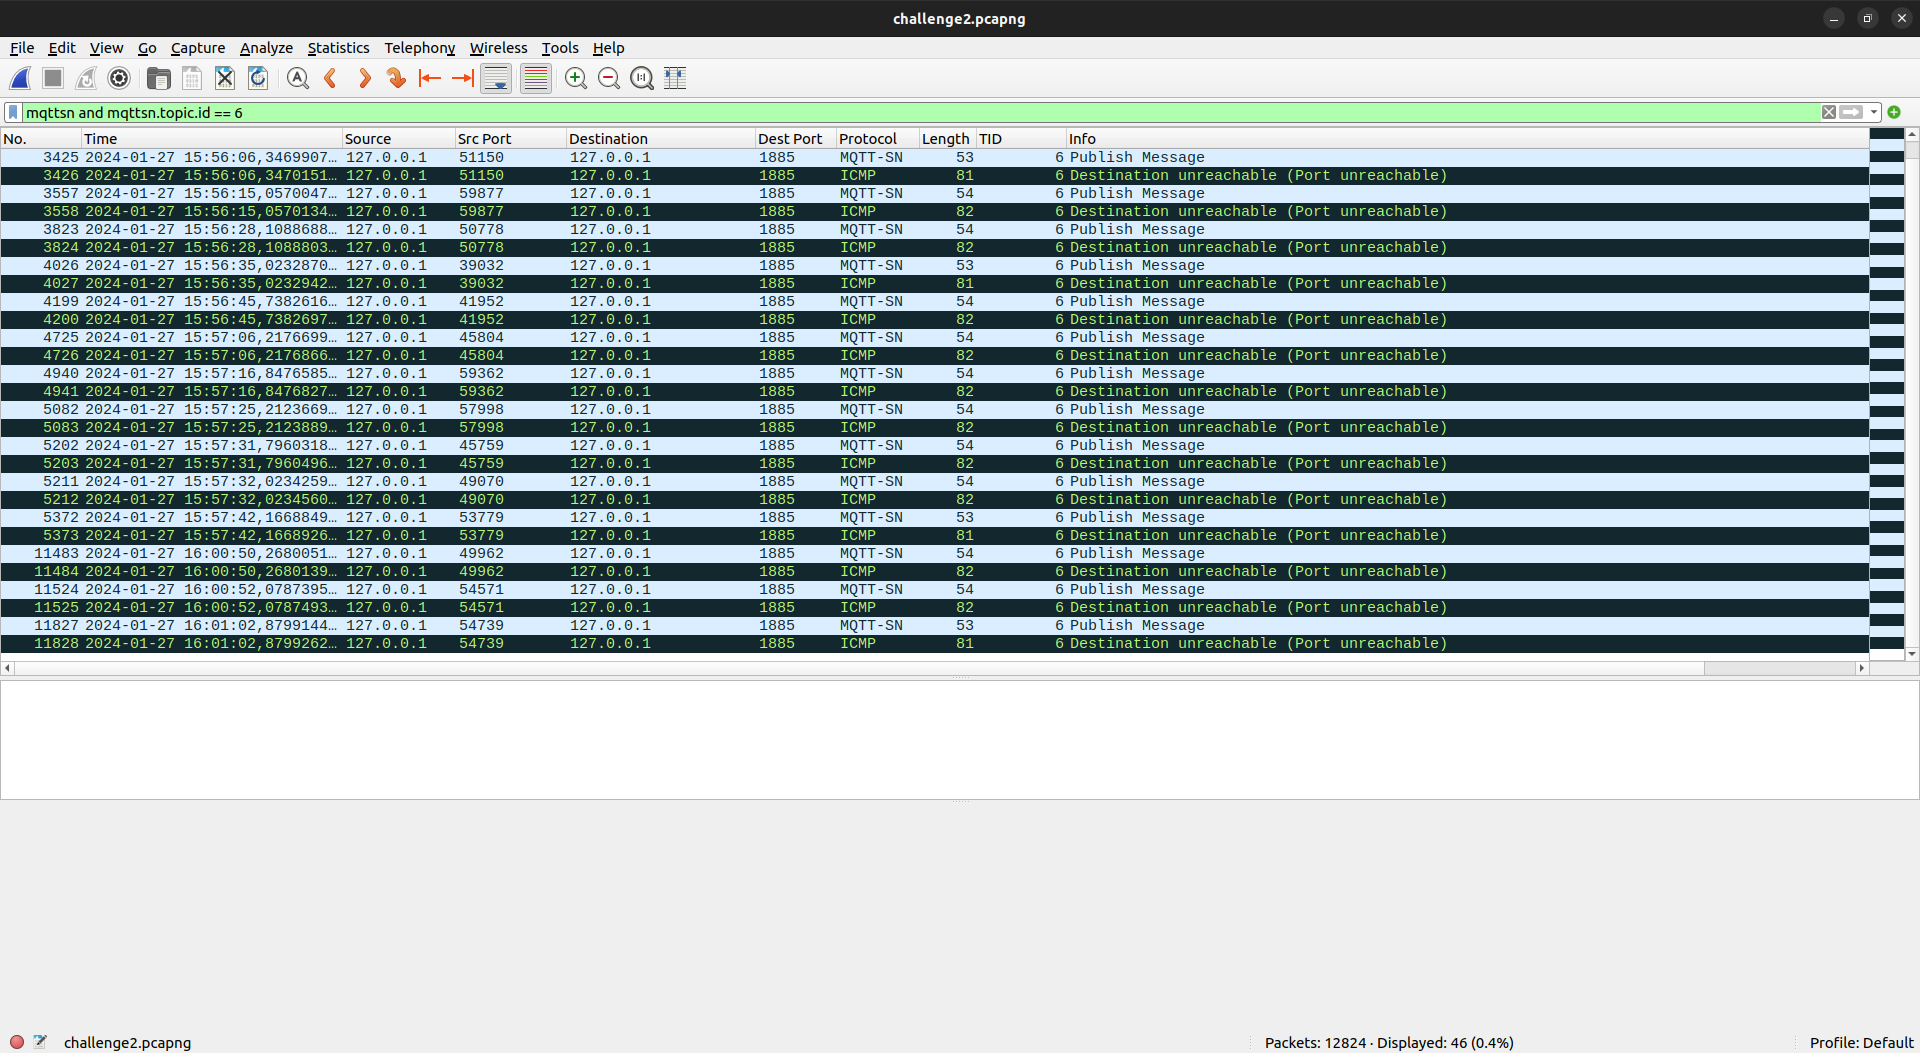
\includegraphics{7b.png}


    % Add a bibliography block to the postdoc
    
    
    
\end{document}
